\documentclass{beamer}

\usepackage{amsmath}
\usepackage{amssymb}
\usepackage{booktabs}
\usepackage{rotating}
\usepackage{multirow}
\usepackage{colortbl,color}
\usepackage{graphics}
\usepackage{sgame}
\usepackage{epstopdf}
\usetheme{default}
%\setbeamercovered{transparent}


\defbeamertemplate{itemize subitem}{dash}{--}
\defbeamertemplate{itemize subsubitem}{dash}{--}
\setbeamertemplate{itemize item}[circle]
\setbeamertemplate{itemize subitem}[dash]
\setbeamertemplate{itemize subsubitem}[dash]
\setbeamertemplate{enumerate item}{\arabic{enumi}.}
\setbeamertemplate{enumerate subitem}{(\alph{enumii})}
\usefoottemplate{}

\newcommand{\showOn}[3]{\only<#2>{\color<#2>{black} #1}\only<#3>{\color<#3>{white} #1}}

\setbeamertemplate{headline}{}
\usenavigationsymbolstemplate{}
\setbeamercolor{titlelike}{fg=black}
\setbeamercolor{item}{fg=black}

\begin{document}
\section{Intro}
\title{Experiments on Communication }
\author{Alistair J. Wilson }
\date{Stanford 2016}
 \maketitle

\begin{frame}{Communication Intro}
	\begin{itemize}
		\item Communication:
		\begin{enumerate}
			\item Coordination
			\item Information Transmission
			\item Analogy \& Instruction
		\end{enumerate}
	\end{itemize}
\end{frame}

\begin{frame}{Cheap Talk (Farrell \& Rabin JEP 1996)}
	\begin{itemize}
		\item Broad overview article on the theory of communication and cheap talk
		\item Outline natural language as a coordination device
	\end{itemize}
\end{frame}

\begin{frame}{Cheap Talk (Farrell \& Rabin JEP 1996)}
	\begin{itemize}
		\item Define some terms:
		\begin{itemize}
			\item Self-committing
			\item Self-signaling
		\end{itemize}
	\end{itemize}
\end{frame}

\begin{frame}
 \textbf{Self-committing:}
		\begin{itemize}
			\item This is when the message, if it succeeds in persuading the other players, makes it optimal to take the advocated action
			\item For example: Any message which has other players follow the Nash Equilibrium is necessarily self-committing.
		\end{itemize}
\end{frame}

\begin{frame}
\textbf{Self-signaling:}
		\begin{itemize}
			\item The message action induces behavior in others (if believed) that is optimal for the sender if and only if the sender takes the action she is advocating.
			\item For example: Coordination in a Battle of the Sexes Game
		\end{itemize}
\end{frame}

\begin{frame}{Multiple Equilibria...}
	\begin{itemize}
		\item Note that the Stag-hunt game is not self-signaling!
		\item Those hunting Hares would also prefer the other agent to choose to hunt a Stag
		\item So a message of ``Let's Hunt Stag'' is \emph{self-committing}, but not \emph{self-signaling}
		\item A message of ``Let's Hunt hare'' is both \emph{self-committing} and \emph{self-signaling}
	\end{itemize}
\end{frame}

\begin{frame}{Coordination}
	\begin{itemize}
		\item We will look at two types of coordination. Games in which the equilibria are :
		\begin{itemize}
			\item not Pareto-ranked (think Battle of the Sexes)
			\item Pareto-ranked (think Stag-hunt)
		\end{itemize}
	\end{itemize}
\end{frame}


\begin{frame}{Battle of the Sexes}
From Cooper, DeJong, Forsythe and Ross (Rand 1989).
\begin{center}
Payoff Table $(x>y>0)$:

		\begin{tabular}{r|c|c|}
				\multicolumn{1}{r}{}& \multicolumn{1}{c}{$c_1$}  & \multicolumn{1}{c}{$c_2$} \\ \cline{2-3}
				$r_1$ &  $0,0$ & $y,x$ \\ \cline{2-3}
				$r_2$ &  $x,y$ & $0,0$ \\ \cline{2-3}
				\end{tabular}
\end{center}

	\begin{itemize}
		\item This has three equilibria:
			\begin{itemize}
				\item $(r_1,c_2)$
				\item $(r_2,c_1)$
				\item Mixed strategy: $\tfrac{x}{x+y}$\% on strategy 2.
			\end{itemize}
	\end{itemize}
\end{frame}

\begin{frame}{Battle of the Sexes (Rand 1989)}
	\begin{itemize}
		\item Think of this as an entry game
		\item Two firms, in a nearby industry have to decide whether to enter a new industry
		\item But, the new industry is a natural monopoly
		\item Each prefers that they be the monopolist, but both entering, or neither entering are the worst outcomes
		\item But if we think of firms as entirely symmetric, it seems strange to focus on the efficient asymmetric outcomes
	\end{itemize}
\end{frame}

\begin{frame}{Battle of the Sexes (Rand 1989)}
	\begin{itemize}
		\item If we actually think of the choice of a couple deciding where to go, then it's obvious that communication is involved
		\item But, even in the entry game example, announcements of intent, \emph{etc.} seem like they would do the same thing
		\item Communication can serve to provide a public randomization device to allow for correlated equilibria.
	\end{itemize}
\end{frame}

\begin{frame}{Battle of the Sexes (Rand 1989)}
	\begin{itemize}
		\item Suppose each player has two messages $\diamond$ and $\circ$
		\item Think of the communication between each player as a simultaneous choice
		\item As in the matching pennies game, let $(\diamond,\diamond)$ and $(\circ,\circ)$  mean that \emph{Row} enters
		\item If the messages are $(\diamond,\circ)$ or $(\circ,\diamond)$ then \emph{Col} enters
	\end{itemize}
\end{frame}

\begin{frame}{Battle of the Sexes (Rand 1989)}
	\begin{itemize}
		\item But this seems a little like the initial problem...
		\item Why would we assume two actors who were unable to coordinate on an equilibrium are suddenly able to coordinate on this communication pre-game?
		\item Natural language is a much more focal idea
		\item So each instead will send a message for one option
	\end{itemize}
\end{frame}

\begin{frame}{Battle of the Sexes (Rand 1989)}
	\begin{itemize}
		\item Maybe one player gets to move first, and therefore can credibly signal that they will enter
		\item In this sense, one player is asymmetric, and has the power to make one of the equilibria focal
		\item Or if the announcements are simultaneous, this is more like bargaining...
		\item With a back and forth conversation, this is somewhat like deciding to relent or not and go with the other's preferred option
		\item But this decision to relent is inherently strategic
		\item More rounds of the debate might be better, but more rounds also alters the behavior
	\end{itemize}
\end{frame}

\begin{frame}{Farrel (1987)}
	\begin{itemize}
		\item Suppose there are $2$ periods of arguing.
		\item In each period, the two players simultaneously send a message \emph{``Enter''}, \emph{``Stay Out''} or \emph{``Silence''}.
		\item Coordinated outcomes are:
	\end{itemize}
	\begin{center}
		\begin{tabular}{r|c|c|c|}
				\multicolumn{1}{r}{}& \multicolumn{1}{c}{\emph{Enter}}  & \multicolumn{1}{c}{\emph{Silence}} & \multicolumn{1}{c}{\emph{Stay Out}}\\ \cline{2-4}
				\emph{Enter} &  Mixed & Row  & Row \\ \cline{2-4}
				\emph{Silence} &  Column & Mixed &  Row\\ \cline{2-4}
				\emph{Stay Out} &  Column & Column & Mixed  \\ \cline{2-4}
		\end{tabular}
\end{center}
\end{frame}
\begin{frame}{Farrell (1987)}
	\begin{itemize}
		\item In the last period we can solve for indifference over each message using the Mixed outcome payoff $u=\tfrac{xy}{x+y}$
		\item So the expected payoff in period $T$ is $V_T$
		\item In period $T-1$, the expected payoff from matched messages is $V_T$, so we can now work out the strategies and $V_{T-1}$
		\item So this is like a war of attrition, with an increasing probability of relenting as we get closer to the final outcome
	\end{itemize}
\end{frame}
\begin{frame}{Battle of the Sexes (Rand 1989)}
	\begin{itemize}
		\item Set-up:
		\begin{itemize}
			\item Undergrads and MBAs from University of Iowa
			\item 11 subjects in a session
			\begin{itemize}
				\item Everyone plays everyone else once
				\item One player sits out every round
			\end{itemize}
			\item Lottery method in every round for prizes (\$1 or \$2)
			\item $x=600$, $y=200$ ($\Longrightarrow u=150, \Pr\left\{\text{Eqbm}\right\}$)
			\item First 10 periods play a dominant-strategy game
			\item Then twenty periods of treatment BoS game
		\end{itemize}
	\end{itemize}
\end{frame}

\begin{frame}{Battle of the Sexes (Rand 1989)}
	\begin{itemize}
		\item Four treatments
		\begin{itemize}
			\item No Communication
			\item One-way communication
			\item Two-way communication (1 round)
			\item Two-way communication (3 rounds)
		\end{itemize}
		\item Main assessment metric is fraction of (pure) equilibrium outcomes
	\end{itemize}
\end{frame}

\begin{frame}{Battle of the Sexes (Rand 1989)}
	\begin{itemize}
		\item Data pooled across sessions
	\end{itemize}
	\begin{center}
		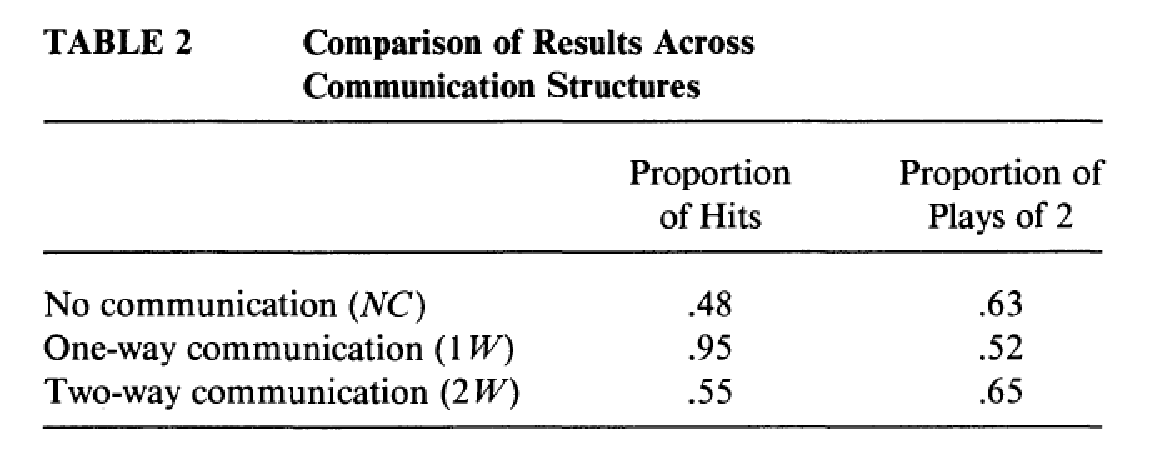
\includegraphics[width=3.0in]{./images/cdfr1989Tbl2.eps}
	\end{center}
		\begin{itemize}
			\item Baseline Hits in Mixed Eqbm is 0.375
			\item In Farrell model with one two-way round 0.499
		\end{itemize}
\end{frame}

\begin{frame}{Battle of the Sexes (Rand 1989)}
	\begin{itemize}
		\item Examining the one-way communication
	\end{itemize}
	\begin{center}
		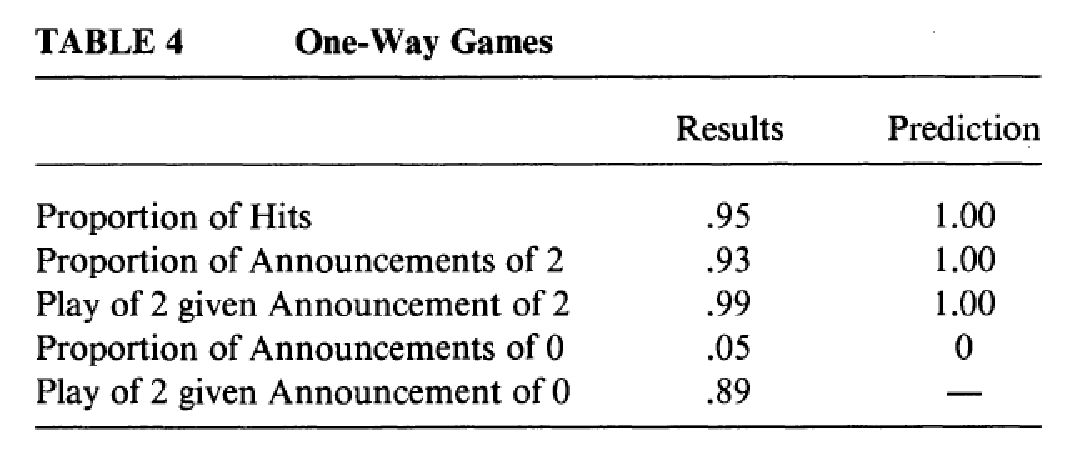
\includegraphics[width=3.0in]{./images/cdfr1989Tbl4.eps}
	\end{center}
\end{frame}
\begin{frame}{Battle of the Sexes (Rand 1989)}
	\begin{itemize}
		\item Examining the two-way communication
	\end{itemize}
	\begin{center}
		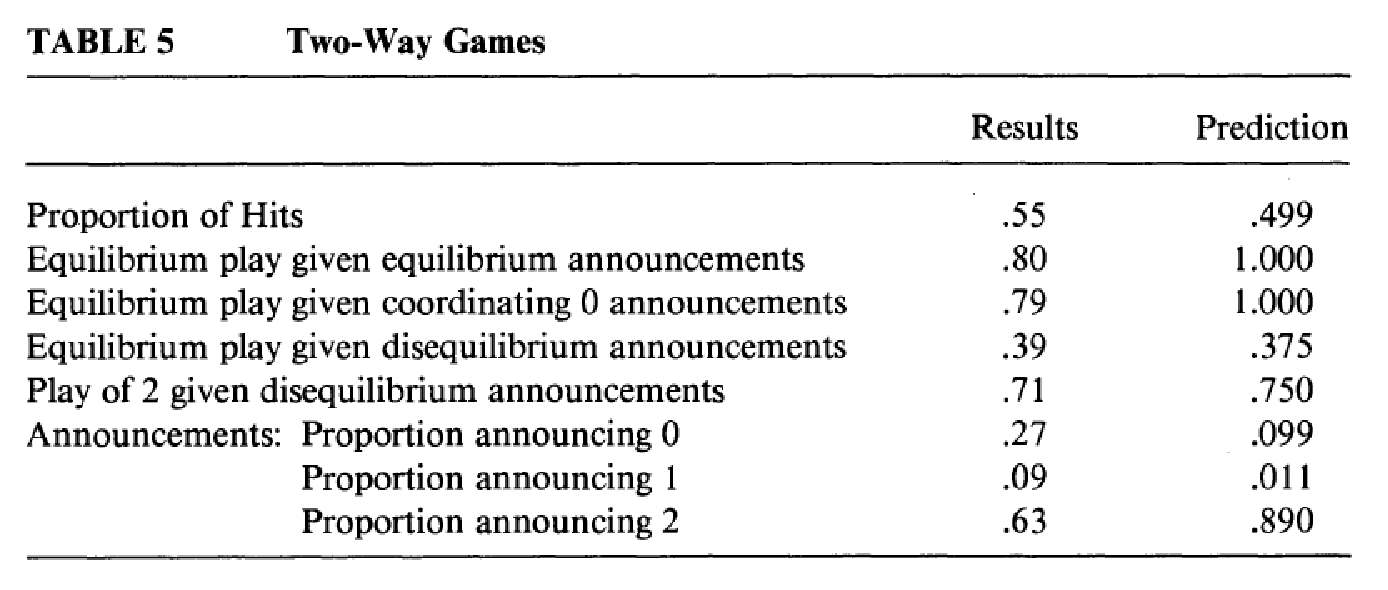
\includegraphics[width=3.0in]{./images/cdfr1989Tbl5.eps}
	\end{center}
	``In'' was behavioral best response, followed by silence (282, 204, 159)
\end{frame}
\begin{frame}{Battle of the Sexes (Rand 1989)}
	\begin{itemize}
		\item Examining the two-way communication with three rounds
	\end{itemize}
	\begin{center}
		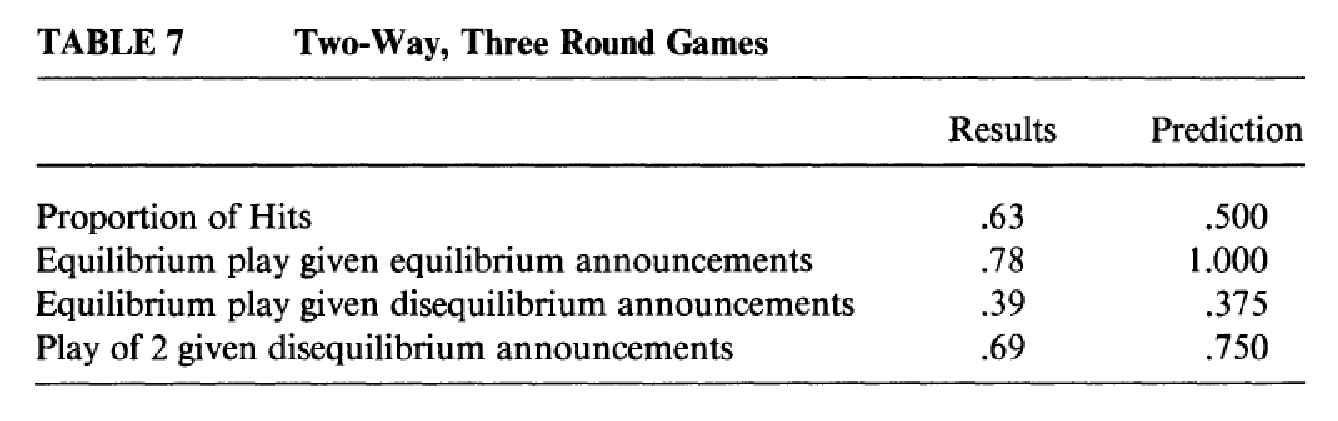
\includegraphics[width=3.0in]{./images/cdfr1989Tbl7.eps}
	\end{center}
	\begin{itemize}
		\item Additional 2 rounds predicted to have only marginal effect
		\item Small increase in Hits observed, up to 0.63 from 0.55
		\item Nowhere near as good as one-way
	\end{itemize}
\end{frame}

\begin{frame}{Battle of the Sexes (Rand 1989)}
	\begin{itemize}
		\item Conclusions:
		\begin{itemize}
			\item Assigning communication power to one individual much more efficient than two-way communication
			\item Focality via communication (as opposed to Schelling)
			\item Extra rounds do slightly better than predicted
			\item Broadly in line with the theory on two-way communication
		\end{itemize}
		\item For me a lot of the details are hidden. Focus is on the efficiency, would like to learn more about individual behavior
	\end{itemize}
\end{frame}

\begin{frame}{Pareto-ranked Equilibria}
	\begin{itemize}
		\item One refinement often used by theorists when dealing with multiple equilibria is to choose the Pareto-superior outcome
		\item But thinking of the stag-hunt game, it is clear that other concerns might dominate (see Harsanyi \& Selten 1988)
		\item Cooper et al. (AER 1990) experimentally demonstrate that coordination at the Pareto-superior equilibrium is not a sure thing
		\begin{itemize}
			\item Risk-dominance (Schmidt, Shupp, Walker and Ostrom GEB 2003)
			\item Optimization-premium effects ( Battalio et al 2001.)
			\item But also payoffs from a dominated strategy can also affect the chosen outcome
		\end{itemize}
	\end{itemize}
\end{frame}

\begin{frame}{Equilibria Selection: Optimization Premium (cf. Battalio et al EMA 2001)}
\begin{center}
\begin{tabular}{r|c|c|}
				\multicolumn{1}{r}{}& \multicolumn{1}{c}{$Y_1$}  & \multicolumn{1}{c}{$Y_2$} \\ \cline{2-3}
				$X_1$ &  $45,45$ & $0,35$ \\ \cline{2-3}
				$X_2$ &  $35,0$ & $40,40$ \\ \cline{2-3}
\end{tabular}
\ \ vs. \
\begin{tabular}{r|c|c|}
				\multicolumn{1}{r}{}& \multicolumn{1}{c}{$Y_1$}  & \multicolumn{1}{c}{$Y_2$} \\ \cline{2-3}
				$X_1$ &  $45,45$ & $0,42$ \\ \cline{2-3}
				$X_2$ &  $42,0$ & $12,12$ \\ \cline{2-3}
\end{tabular}
\end{center}
More people choose $X_1$/$Y_1$ in second game.

(Both games require 80\% belief that other plays strategy one)
\end{frame}

\begin{frame}{Equilibria Selection: Dominated Strategies (cf. Cooper et al 1990)}
	\begin{center}
		\begin{tabular}{r|c|c|c|}
			\multicolumn{1}{r}{ }& \multicolumn{1}{c}{$Y_1$}  & \multicolumn{1}{c}{$Y_2$} & \multicolumn{1}{c}{$Y_3$} \\ \cline{2-4}
			$X_1$ &  $35,35$  & $35,25$  & $100,0$ \\ \cline{2-4}
			$X_2$ &  $25,35$  & $55,55$  & $0,0$   \\ \cline{2-4}
			$X_3$ &  $0,100$  & $0,0$    & $60,60$  \\ \cline{2-4}
		\end{tabular}\ \ vs.\
		\begin{tabular}{r|c|c|c|}
			\multicolumn{1}{r}{ }& \multicolumn{1}{c}{$Y_1$}  & \multicolumn{1}{c}{$Y_2$} & \multicolumn{1}{c}{$Y_3$} \\ \cline{2-4}
			$X_1$ &  35,35 & 35,25  & 100,0 \\ \cline{2-4}
			$X_2$ &  25,35 & 55,55  & 0,0 \\ \cline{2-4}
			$X_3$ &  0,100 & 0,0  & 50,50  \\ \cline{2-4}
		\end{tabular}
	\end{center}

  Removing the cooperative max point allows for coordination at Pareto-dominant equilibrium.
\end{frame}

\begin{frame}{Communication and coordination in Pareto-ranked games}
	\begin{itemize}
		\item Cooper et al. (QJE 1992) examine the effect of cheap-talk on these games
		\item They categorize these games in two ways:
			\begin{itemize}
				\item Simple coordination games (SCG)
				\item Cooperative coordination games (CCG)
			\end{itemize}
		\item By SCG they mean Stag-hunt type-games, and by CCG those games with a non-equilibrium efficient outcome
	\end{itemize}
\end{frame}

\begin{frame}{Cooper et al. (QJE 1992)}
	\begin{itemize}
		\item SCG game is:
		\begin{center}
		\begin{tabular}{r|c|c|}
				\multicolumn{1}{r}{}& \multicolumn{1}{c}{$Y_1$}  & \multicolumn{1}{c}{$Y_2$} \\ \cline{2-3}
				$X_1$ &  $800,800$ & $800,0$ \\ \cline{2-3}
				$X_2$ &  $0,800$ & $1000,1000$ \\ \cline{2-3}
\end{tabular}
\end{center}
		\item CCG game is:
		\begin{center}
			\begin{tabular}{r|c|c|c|}
				\multicolumn{1}{r}{ } & \multicolumn{1}{c}{$Y_1$}  & \multicolumn{1}{c}{$Y_2$} & \multicolumn{1}{c}{$Y_3$} \\ \cline{2-4}
				$X_1$ &  350,350 & 350,250  & 1000,0 \\ \cline{2-4}
				$X_2$ &  250,350 & 550,550  & 0,0 \\ \cline{2-4}
				$X_3$ &  0,1000 & 0,0  & 600,600  \\ \cline{2-4}
			\end{tabular}
		\end{center}
	\end{itemize}
\end{frame}

\begin{frame}{Cooper et al. (QJE 1992)}
	\begin{itemize}
		\item Treatments are factorial design of:
			\begin{enumerate}
				\item SCG game or CCG game
				\item No communication, one-way communication, or two-way communication
			\end{enumerate}
	\end{itemize}
\end{frame}

\begin{frame}{Cooper et al. (QJE 1992)}
	Equilibrium results $(X_2,Y_2)$ outcome
			\begin{center}
			\begin{tabular}{lccc}
			\hline & No Comm & One-Way Comm & Two-way Comm \\ \hline
			SCG    &  0.0\%	 & 53.3\%       &  90.9\% \\
			CCG    &  3.0\%	 & 67.3\%       &  29.1\%
			\\\hline
			\end{tabular}\end{center}
		\begin{itemize}
			\item Two-way communication is necessary to overcome risk-dominant strategy in stag-hunt game
			\item But less effective in CCG game than one-way
		\end{itemize}
\end{frame}

\begin{frame}{Cooper et al. (QJE 1992)}
\begin{center}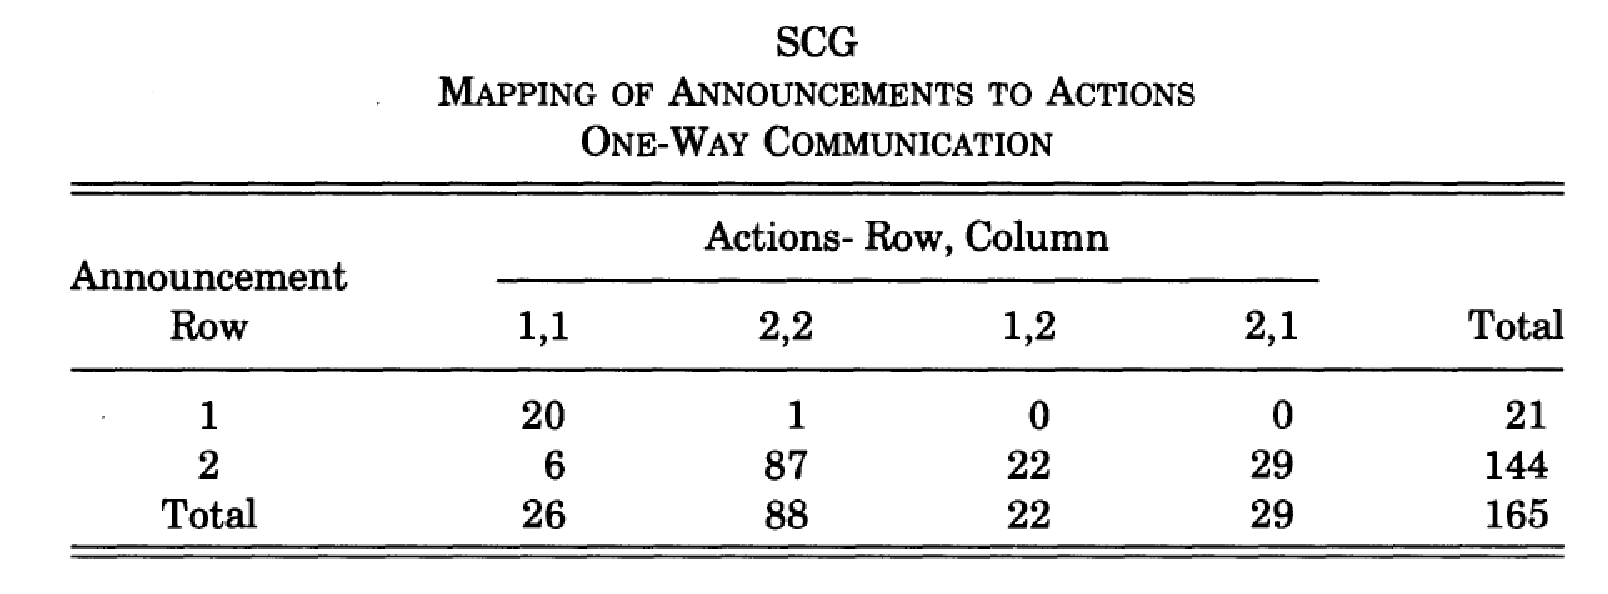
\includegraphics[width=3.0in]{./images/cdfr1992Tbl2.eps}\end{center}
	\begin{itemize}
		\item Most messages are coordinating on the pareto-dominant symmetric equilibrium
		\item But those receiving messages only play strategy $2$  about 75\% of the time.
		\item Need greater than 80\% chance for a risk-nuetral agent to choose $2$
		\item Those sending $2$ choose that strategy 80.6\% of the time
	\end{itemize}
\end{frame}

\begin{frame}{Cooper et al. (QJE 1992)}
\begin{center}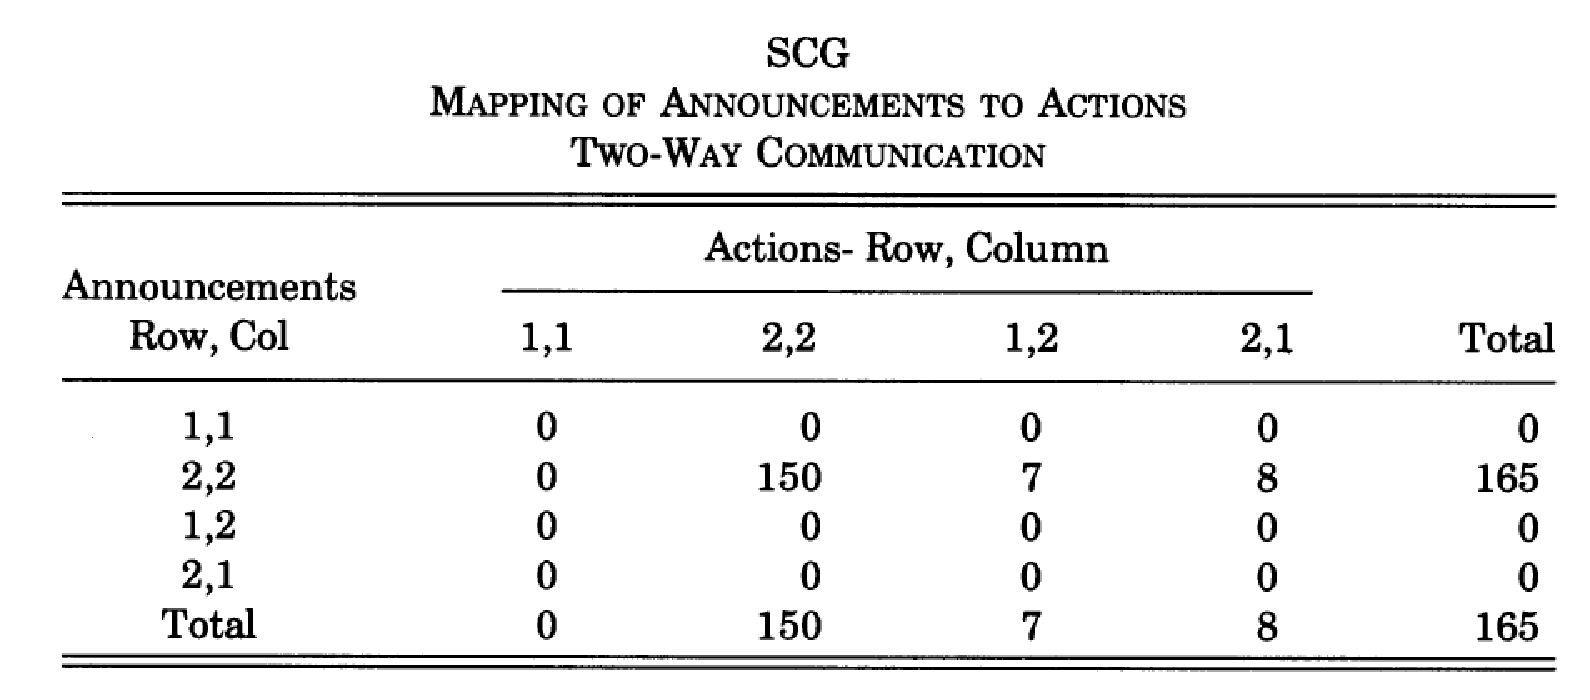
\includegraphics[width=3.0in]{./images/cdfr1992Tbl3.eps}\end{center}
	\begin{itemize}
		\item \textbf{All} messages are coordinating on the pareto-dominant symmetric equilibrium
		\item 95.6\% of choice are for 2
		\item No outcomes at pareto-inferior equilibrium
	\end{itemize}
\end{frame}
\begin{frame}{Cooper et al. (QJE 1992)}
\begin{center}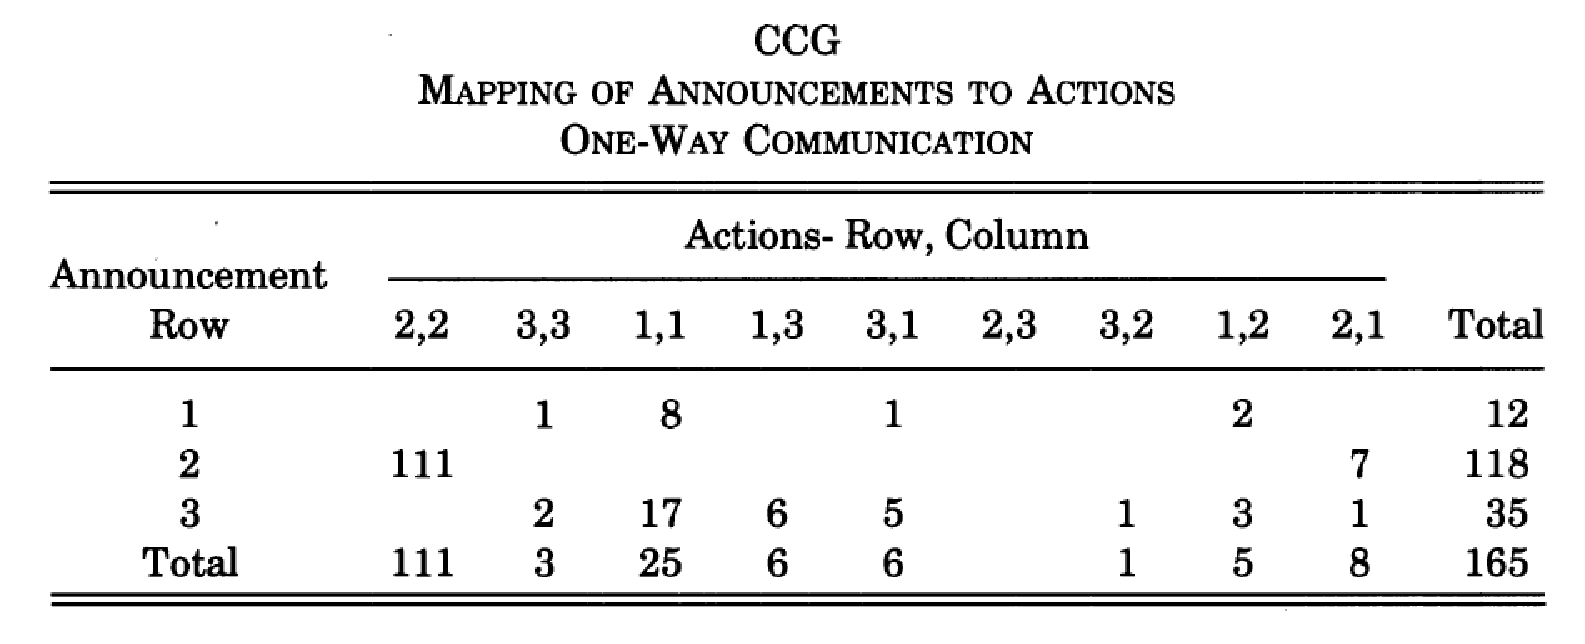
\includegraphics[width=3.0in]{./images/cdfr1992Tbl5.eps}\end{center}
	\begin{itemize}
		\item 67.2\% of one-way messages are for the pareto-dominant symmetric equilibrium
		\item ... 94.1\% of the time yielding the pareto-dominant outcome
		\item Messages for 3 are mostly fool's gold (sender's play 1 80\% of the time!)
	\end{itemize}
\end{frame}
\begin{frame}{Cooper et al. (QJE 1992)}
\begin{center}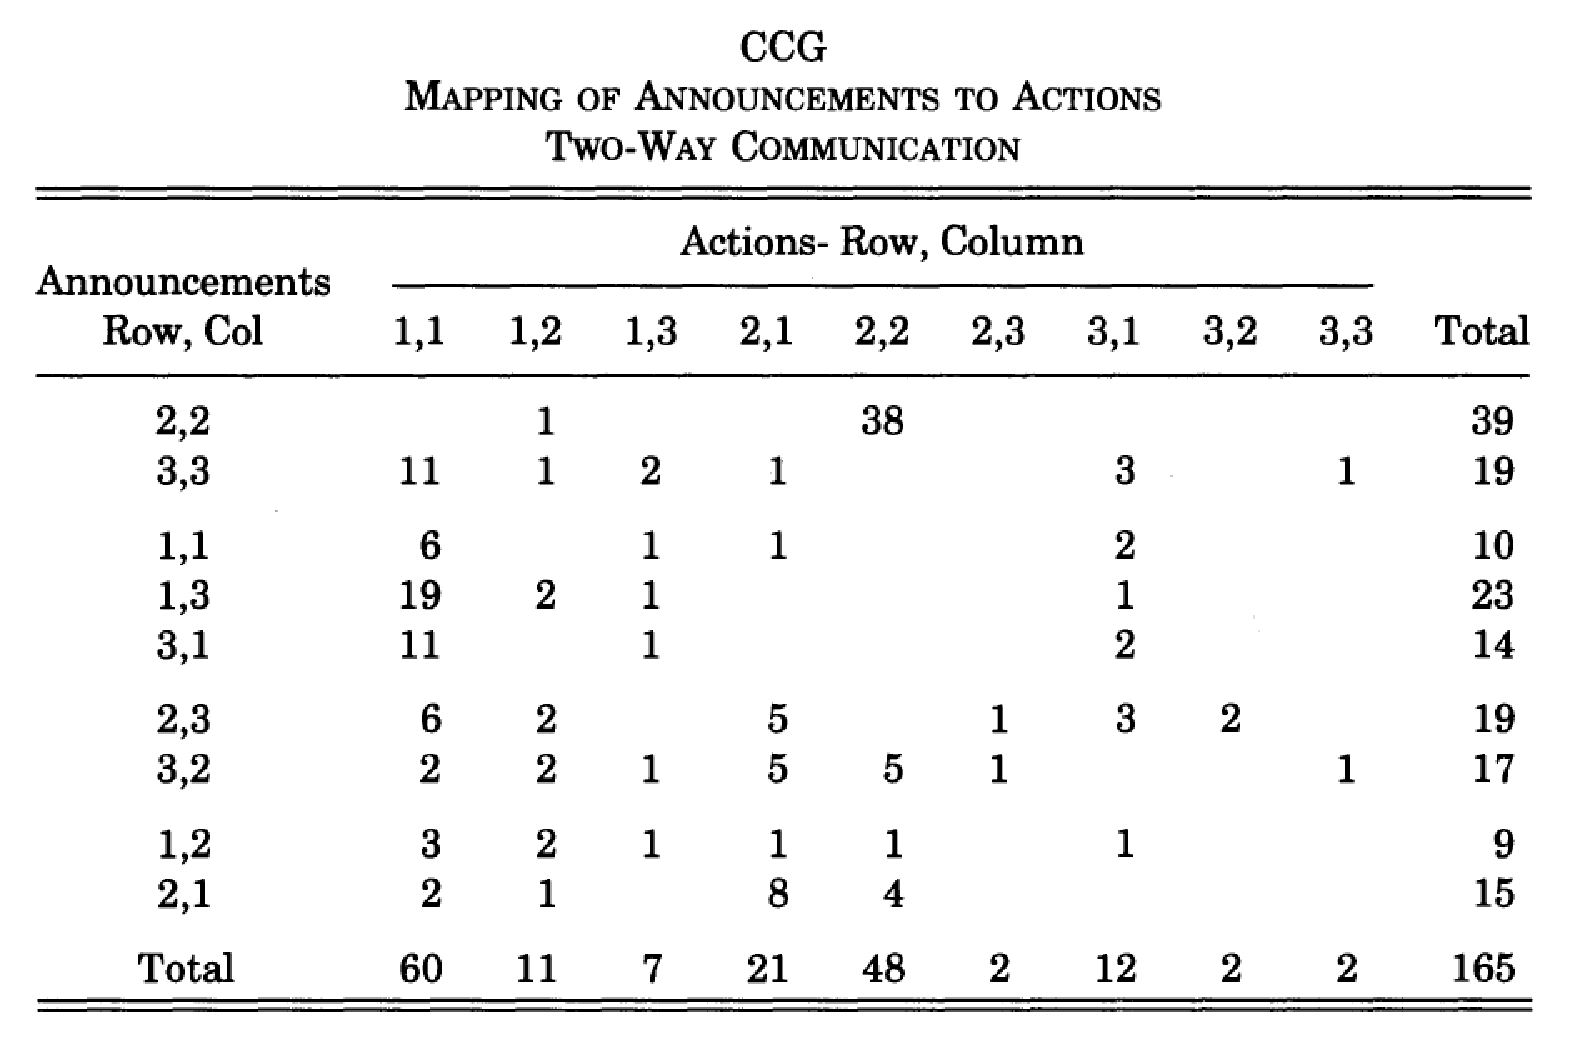
\includegraphics[width=3in]{./images/cdfr1992Tbl6.eps}\end{center}
	\begin{itemize}
		\item $(2,2)$ announcements are great for coordinating (38/39)
		\item Messages \textbf{for} the cooperative outcome mostly yield the pareto-inferior equilibrium outcome
	\end{itemize}
\end{frame}
\begin{frame}{Cooper et al. (QJE 1992)}
	\begin{itemize}
		\item Authors fit an explanatory model with ``altruists'' and ``egoists''
		\item Binary model of other-regarding preference
		\item Altruists want to play the (3,3) outcome, but egoists want the cash
		\item Communication that could allow equilibrium coordination gets co-opted for coordination in the prisoner's dilemma part
		\item Attempt to test model through selection of selfish or altruistic subjects from a dictator game. Mixed results for altrusits. Egoists are still selfish.
	\end{itemize}
\end{frame}

\begin{frame}{Duffy and Feltovich (2002)}
\begin{itemize}
 \item Primary motivation is coordination/efficiency
 \item Look at three games and ask what is better:
	 \begin{itemize}
		 \item Cheap Talk
		 \item Observation
		 \item Experience
	\end{itemize}
\end{itemize}
\end{frame}


\begin{frame}{Duffy and Feltovich (2002)}

\begin{center}
\begin{tabular}{r|c|c|}
				\multicolumn{1}{r}{}& \multicolumn{1}{c}{$C_2$}  & \multicolumn{1}{c}{$D_2$} \\ \cline{2-3}
				$C_1$ &  $70,70$ & $10,80$ \\ \cline{2-3}
				$D_1$ &  $80,10$ & $40,40$ \\ \cline{2-3}
\end{tabular}
\begin{tabular}{r|c|c|}
				\multicolumn{1}{r}{}& \multicolumn{1}{c}{$C_2$}  & \multicolumn{1}{c}{$D_2$} \\ \cline{2-3}
				$C_1$ &  $70,70$ & $10, 55$ \\ \cline{2-3}
				$D_1$ &  $55,10$ & $55,55$ \\ \cline{2-3}
\end{tabular}
\begin{tabular}{r|c|c|}
				\multicolumn{1}{r}{}& \multicolumn{1}{c}{$C_2$}  & \multicolumn{1}{c}{$D_2$} \\ \cline{2-3}
				$C_1$ &  $70,70$ & $50,80$ \\ \cline{2-3}
				$D_1$ &  $80,50$ & $40,40$ \\ \cline{2-3}
\end{tabular}
\end{center}

\end{frame}

\begin{frame}{Duffy and Feltovich (2002)}
\begin{itemize}
	\item Three games, run within
		\begin{itemize}
			\item Prisoner's Dilemma
			\item Stag Hunt
			\item Chicken
		\end{itemize}
	\item Vary between
		\begin{itemize}
			\item Cheap Talk Observation
			\item Play Observation
			\item Nothing
		\end{itemize}
	\end{itemize}
\end{frame}

\begin{frame}{Duffy and Feltovich (2002)}
\begin{itemize}
	\item Lottery method, points are percentage chance of winning dollar
	\item Do not exhaust all within-subject orders (just run 2, SH in middle)
	\item 10 rounds each game
	\item 50-50 chance of being selected to be sender
\end{itemize}
\end{frame}

\begin{frame}{Duffy and Feltovich (2002)}
\begin{center}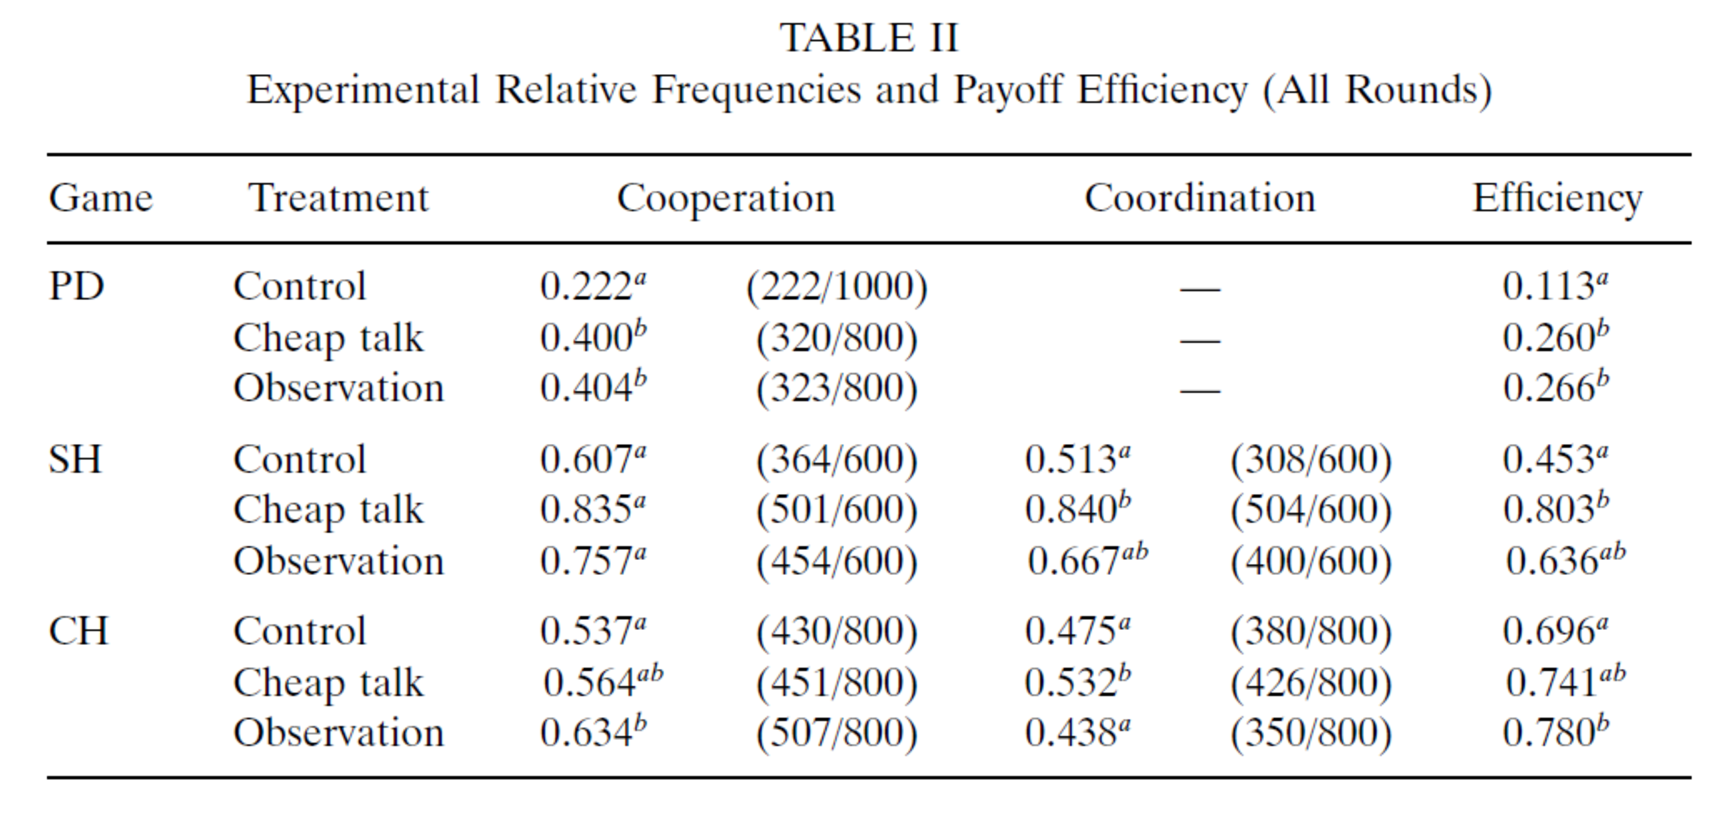
\includegraphics[width=4.0in]{./images/df2002tbl2.eps}\end{center}
\end{frame}

\begin{frame}{Duffy and Feltovich (2002)}
\begin{center}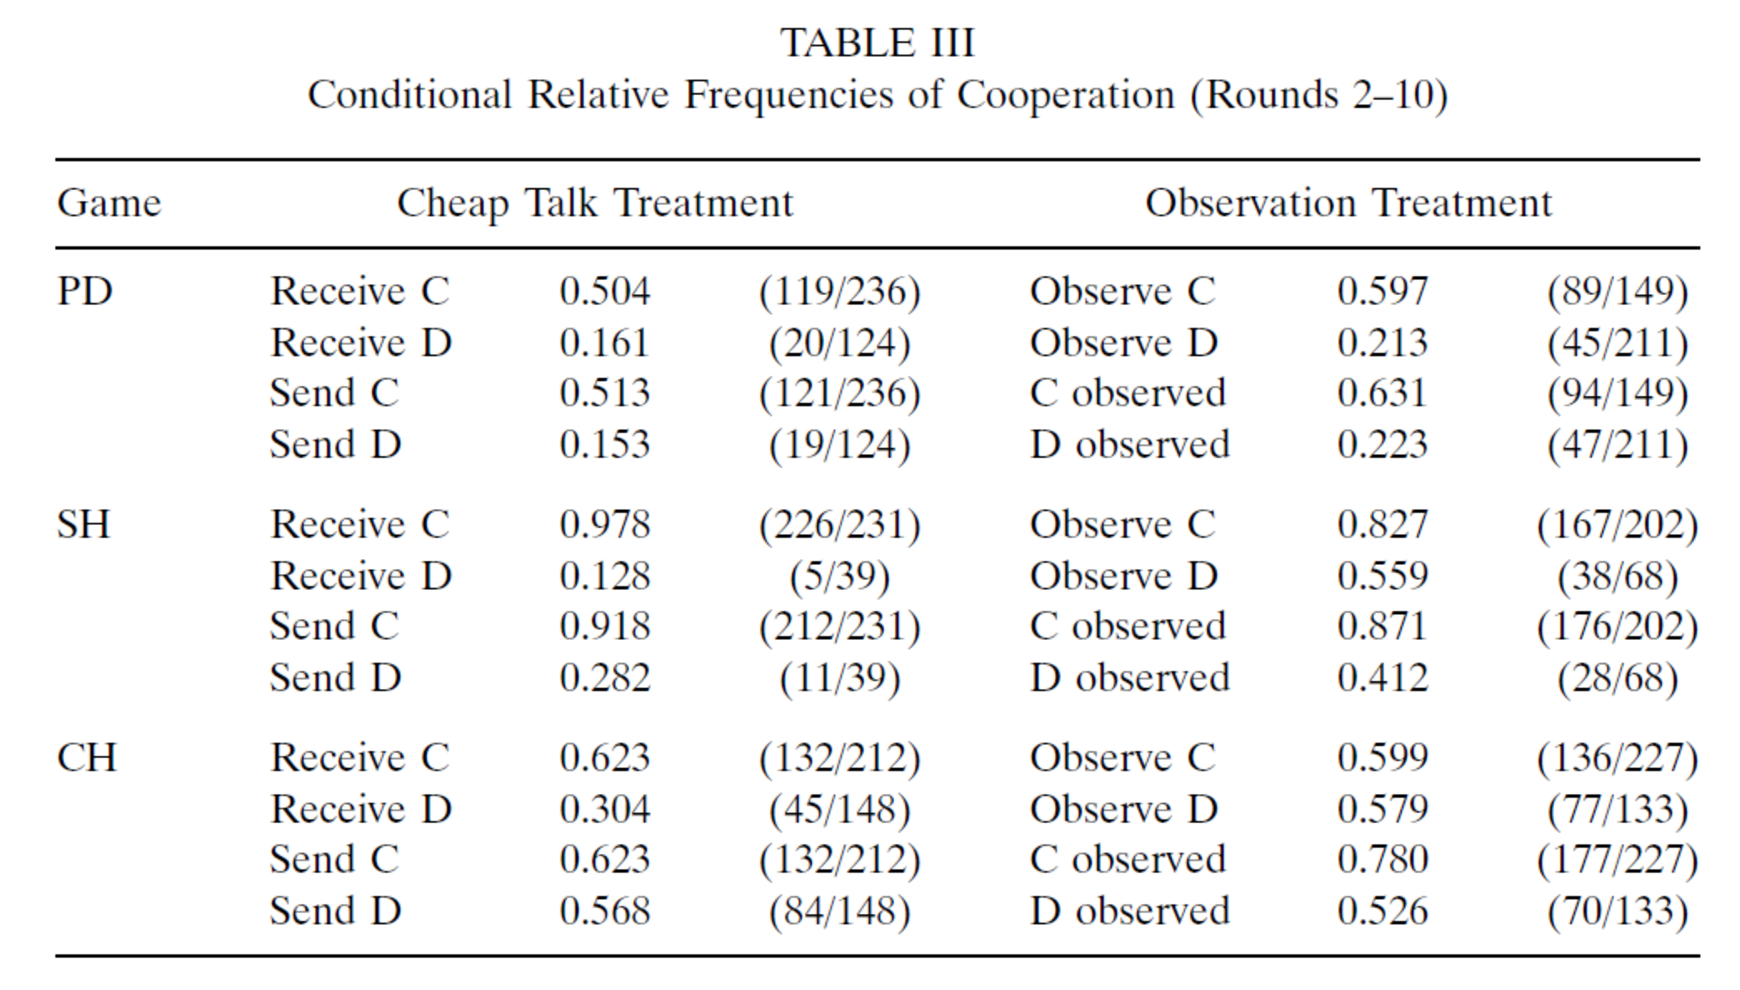
\includegraphics[width=4.0in]{./images/df2002tb3.eps}\end{center}
\end{frame}

\begin{frame}{Duffy and Feltovich (2002)}
\begin{itemize}
	\item Conclude that both observation and cheap talk useful
	\item Cheap Talk better in games where common interest in coordination
	\item Observation better in PD and Chicken. (I would say this is more mixed)
\end{itemize}
\end{frame}

\begin{frame}{Communication Intro}
	\begin{itemize}
		\item Communication:
		\begin{enumerate}
			\item Coordination
			\item \textbf{Information Transmission}
			\item Analogy \& Instruction
		\end{enumerate}
	\end{itemize}
\end{frame}
\section{Intro}
\begin{frame}{ }
	\begin{itemize}
		\item Information Transmission:
			\begin{enumerate}
				\item One player has information on a state of the world $\theta\in\Theta$
				\item \textbf{Sends} a message $m$ to an uninformed player
				\item Uninformed player \textbf{receives} the message and makes a choice $x\in X$
			\end{enumerate}

		\item General preferences are given by $u_S(\theta,m,x)$ and $v_R(\theta,m,x)$
	\end{itemize}
\end{frame}

\begin{frame}{ }
	\begin{itemize}
		\item The solution concept is therefore Bayesian Nash Equilibrium...
		\item ... or a refinement of it:
		\begin{itemize}
			\item Sequential Equilibrium
			\item Perfect Equilibrium
			\item Intuitive Criterion
			\item Divinity \& D1 etc.
			\item Stability
		\end{itemize}
		\item See Kreps\&Wilson EMA 82, Cho\&Kreps QJE 87, Kohlberg\&Mertens EMA 86, etc. for theory
		\item See Banks, Camerer \& Porter (GEB 96) for experimental analysis of these refinements
	\end{itemize}
\end{frame}
\begin{frame}{}
	\begin{itemize}
		\item This sender-receiver framework is fairly general
		\item We will look at cheap-talk here
			\begin{itemize}
				\item $u(\theta,m,x)=u(\theta,m^\prime,x)$ and $v(\theta,m,x)=v(\theta,m^\prime,x)$
				$\forall m,m^\prime\in M$
				\item $M(\theta)=M,\forall\theta\in\Theta$
				\item $X(\theta,m)=X,\forall\theta\in\Theta,\forall m\in M$
			\end{itemize}
		\item All possible messages therefore:
			\begin{itemize}
				\item do not directly affect payoffs
				\item do not restrict the action set
				\item are available for all states
			\end{itemize}
		\item So we eliminate costly signaling games (e.g. the Spence model)
		\item And verifiable messages (Milgrom \& Roberts Rand `86)
	\end{itemize}
\end{frame}

\section{Crawford \& Sobel (EMA 1982)}
\begin{frame}{Crawford \& Sobel (EMA 1982)}
	\begin{itemize}
		\item State $\theta$ drawn on interval $\Theta$ according to some distribution
		\item Receiver preferences over action $x\in X=\Theta$ are $$v^R(x,\theta)=-\left\|x-\theta \right\|$$
		\item Sender preferences are $$u^S(x,\theta)=-\left\|x+b-\theta \right\|$$
		where $b$ is the preference misalignment
		\item Timing
		\begin{enumerate}[i)]
		\item State $\theta$ drawn, Sender observes
		\item Sender chooses message $m\in M$
		\item Receiver observes $m$, choose action $x$
		\end{enumerate}
	\end{itemize}
\end{frame}

\begin{frame}{Crawford-Sobel Example}
	\begin{center}
		\includegraphics<1>[width=1.0\textwidth]{images/CSexample-1.eps}
		\includegraphics<2>[width=1.0\textwidth]{images/CSexample-2.eps}
		\includegraphics<3-5>[width=1.0\textwidth]{images/CSexample-3.eps}
		\includegraphics<6>[width=1.0\textwidth]{images/CSexample-9.eps}
		\includegraphics<7>[width=1.0\textwidth]{images/CSexample-10.eps}
		\includegraphics<8>[width=1.0\textwidth]{images/CSexample-11.eps}
		\includegraphics<9>[width=1.0\textwidth]{images/CSexample-12.eps}
		\includegraphics<10>[width=1.0\textwidth]{images/CSexample-13.eps}
		\includegraphics<11>[width=1.0\textwidth]{images/CSexample-14.eps}
	\end{center}

	\only<1-2>{State realized}
	\only<3>{Sender has optimal point $b$ to right of $\theta$}
	\only<4>{Sender sends a message $m(\theta)$}
	\only<5>{Receiver makes a choice $x(m)$, optimal point of $\theta$}
	\only<6>{Sender could reveal truth with $m(\theta)=\theta$.}
	\only<7>{In which case the Receiver chooses their best point}
	\only<8>{Not an equilibrium, as now the sender exaggerates...}
	\only<9>{...to which the receiver reacts...}
	\only<10>{...and on...}
	\only<11>{...and on.}
\end{frame}

\begin{frame}{Crawford-Sobel Equilibrium}
	\begin{center}
		\includegraphics<1>[width=1.0\textwidth]{images/CSexample-Eq1.eps}
		\includegraphics<2>[width=1.0\textwidth]{images/CSexample-Eq1b.eps}
		\includegraphics<3>[width=1.0\textwidth]{images/CSexample-Eq2.eps}
		\includegraphics<4>[width=1.0\textwidth]{images/CSexample-Eq2b.eps}
		\includegraphics<5>[width=1.0\textwidth]{images/CSexample-Eq3.eps}
		\includegraphics<6-8>[width=1.0\textwidth]{images/CSexample-Eq3b.eps}
	\end{center}

	\only<1-2>{Babbling, meaningless message}
	\only<3-4>{Partial Revelation, like ``Low'' or ``High''}
	\only<5-6>{Partial Revelation, Like ``Low'', ``Medium'' or ``High''}
	\only<7>{More messages are more informative}
	\only<8>{Message identities are meaningless}


\end{frame}
\section{Dickhaut, McCabe Mukherji (ET 1994)}
\begin{frame}{Dickhaut, McCabe Mukherji (ET 1994)}
	\begin{itemize}
		\item Four possible states $\Theta=\left\{1,2,3,4 \right\}$
		\item Four possible actions $X=\left\{1,2,3,4 \right\}$
		\item Preferences of the receiver are:
				$$v^R(x,\theta)=C_R-a\cdot \left|x-\theta\right|^{1.1}$$
				and for the sender are:
				$$u^S(x,\theta;b)=C_S-a\cdot \left|x-\theta-b\right|^{1.1}$$
		\item Treatment variable is $-b$, which takes on values in $\left\{0.25,0.5,1.0,2.0,3.0\right\}$
	\end{itemize}
\end{frame}

\begin{frame}{Dickhaut, McCabe Mukherji (ET 1994)}
Treatment with $b=0.25$ (\emph{Sender},\emph{Receiver})

\begin{center}
	\begin{tabular}{r|c|c|c|c|}
			\multicolumn{1}{r}{ }& \multicolumn{4}{c}{State:}		\\
			\multicolumn{1}{r}{ }& \multicolumn{1}{c}{$\theta=1$}  & \multicolumn{1}{c}{$\theta=2$} & \multicolumn{1}{c}{$\theta=3$}& \multicolumn{1}{c}{$\theta=4$} \\ \cline{2-5}
			$x=1$ &  $206,274$ & $176,214$  & $108,145$ & $37,73$  \\ \cline{2-5}
			$x=2$ &  $143,214$ & $206,274$  & $176,214$ & $108,145$ \\ \cline{2-5}
			$x=3$ &  $73,145$  & $143,214$  & $206,274$ & $176,214$  \\ \cline{2-5}
			$x=4$ &  $0,73$    & $73,145$   & $143,214$ & $206,274$    \\ \cline{2-5}
		\end{tabular}
	\end{center}
\end{frame}

\begin{frame}{Dickhaut, McCabe Mukherji (ET 1994)}
Treatment with $b=0.5$ (\emph{Sender},\emph{Receiver})

\begin{center}
	\begin{tabular}{r|c|c|c|c|}
			\multicolumn{1}{r}{ }& \multicolumn{4}{c}{State:}		\\
			\multicolumn{1}{r}{ }& \multicolumn{1}{c}{$\theta=1$}  & \multicolumn{1}{c}{$\theta=2$} & \multicolumn{1}{c}{$\theta=3$}& \multicolumn{1}{c}{$\theta=4$} \\ \cline{2-5}
			$x=1$ &  $242,274$ & $242,214$  & $176,145$ & $105,73$  \\ \cline{2-5}
			$x=2$ &  $176,214$ & $242,274$  & $242,214$ & $176,145$ \\ \cline{2-5}
			$x=3$ &  $105,145$ & $176,214$  & $242,274$ & $242,214$  \\ \cline{2-5}
			$x=4$ &  $31,73$   & $105,145$  & $176,214$ & $242,274$    \\ \cline{2-5}
		\end{tabular}
	\end{center}
\end{frame}

\begin{frame}{Dickhaut, McCabe Mukherji (ET 1994)}
Treatment with $b=1.0$ (\emph{Sender},\emph{Receiver})

\begin{center}
	\begin{tabular}{r|c|c|c|c|}
			\multicolumn{1}{r}{ }& \multicolumn{4}{c}{State:}		\\
			\multicolumn{1}{r}{ }& \multicolumn{1}{c}{$\theta=1$}  & \multicolumn{1}{c}{$\theta=2$} & \multicolumn{1}{c}{$\theta=3$}& \multicolumn{1}{c}{$\theta=4$} \\ \cline{2-5}
			$x=1$ &  $216,274$ & $276,214$  & $216,145$ & $147,73$  \\ \cline{2-5}
			$x=2$ &  $147,214$ & $216,274$  & $276,214$ & $216,145$ \\ \cline{2-5}
			$x=3$ &  $75,145$  & $147,214$  & $216,274$ & $276,214$  \\ \cline{2-5}
			$x=4$ &  $0,73$    & $75,145$   & $147,214$ & $216,274$    \\ \cline{2-5}
		\end{tabular}
	\end{center}
\end{frame}

\begin{frame}{Dickhaut, McCabe Mukherji (ET 1994)}
Treatment with $b=2.0$ (\emph{Sender},\emph{Receiver})

\begin{center}
	\begin{tabular}{r|c|c|c|c|}
			\multicolumn{1}{r}{ }& \multicolumn{4}{c}{State:}		\\
			\multicolumn{1}{r}{ }& \multicolumn{1}{c}{$\theta=1$}  & \multicolumn{1}{c}{$\theta=2$} & \multicolumn{1}{c}{$\theta=3$}& \multicolumn{1}{c}{$\theta=4$} \\ \cline{2-5}
			$x=1$ &  $224,274$ & $293,214$  & $353,145$ & $293,73$  \\ \cline{2-5}
			$x=2$ &  $152,214$ & $224,274$  & $293,214$ & $353,145$ \\ \cline{2-5}
			$x=3$ &  $77,145$  & $152,214$  & $224,274$ & $293,214$  \\ \cline{2-5}
			$x=4$ &  $0,73$    & $77,145$   & $152,214$ & $224,274$    \\ \cline{2-5}
		\end{tabular}
	\end{center}
\end{frame}

\begin{frame}{Dickhaut, McCabe Mukherji (ET 1994)}
Treatment with $b=3.0$ (\emph{Sender},\emph{Receiver})

\begin{center}
	\begin{tabular}{r|c|c|c|c|}
			\multicolumn{1}{r}{ }& \multicolumn{4}{c}{State:}		\\
			\multicolumn{1}{r}{ }& \multicolumn{1}{c}{$\theta=1$}  & \multicolumn{1}{c}{$\theta=2$} & \multicolumn{1}{c}{$\theta=3$}& \multicolumn{1}{c}{$\theta=4$} \\ \cline{2-5}
			$x=1$ &  $230,274$ & $302,214$  & $371,145$ & $431,73$  \\ \cline{2-5}
			$x=2$ &  $155,214$ & $230,274$  & $302,214$ & $371,145$ \\ \cline{2-5}
			$x=3$ &  $78,145$  & $155,214$  & $230,274$ & $302,214$  \\ \cline{2-5}
			$x=4$ &  $0,73$    & $78,145$   & $155,214$  & $230,274$    \\ \cline{2-5}
		\end{tabular}
	\end{center}
\end{frame}

\begin{frame}{Dickhaut, McCabe Mukherji (ET 1994)}
\begin{itemize}
	\item The message space is the union of:
	\begin{itemize}
		\item $\left\{ 1\right\}$,$\left\{ 2\right\}$,$\left\{ 3\right\}$,$\left\{ 4\right\}$
		\item $\left\{ 1,2\right\}$,$\left\{ 2,3\right\}$,$\left\{ 3,4\right\}$
		\item $\left\{ 1,2,3\right\}$,$\left\{ 2,3,4\right\}$
		\item $\left\{ 1,2,3,4\right\}$
	\end{itemize}
\end{itemize}
\end{frame}

\begin{frame}{Dickhaut, McCabe Mukherji (ET 1994)}
\begin{itemize}
	\item All of the games have a babbling equilibrium
	\item Focus on truthful-language equilibria
	\item Games with $b=0.25$ and $b=0.5$ have a truth-telling equilibrium, as well as other
	\item Game with $b=1.0$ has two meaningful equilibria, welfare ranked
	\item Games with $b=2.0$ and $b=3.0$ have only babbling equilibria
\end{itemize}
\end{frame}

\begin{frame}{Dickhaut, McCabe Mukherji (ET 1994)}
\begin{itemize}
	\item Minnesota undergrads
	\item Nine subjects per session
	\begin{itemize}
		\item 4 Senders
		\item 4 Receivers
		\item 1 monitor: fixed \$20 payment
	\end{itemize}
	\item 12 periods
	\item Between subject design, 3 sessions each treatment
\end{itemize}
\end{frame}

\begin{frame}{Dickhaut, McCabe Mukherji (ET 1994)}
Experimental Round
	\begin{enumerate}
		\item Monitor rolls a die
		\item Informs the senders
		\item Senders circle a message on form
		\item Form is passed to matched receiver (pre-randomized match)
		\item Receiver chooses action
	\end{enumerate}
\end{frame}

\begin{frame}{Dickhaut, McCabe Mukherji (ET 1994)}
Look at average distance from state, $\left|\theta_{it}-x_{it}\right|$
	\begin{center}
		\begin{tabular}{lc}\hline
		Treatment &  Mean Distance \\\hline
		 $b=0.25$ &  0.36 \\
		 $b=0.5$  &  0.35 \\
		 $b=1.0$  &  0.56 \\
		 $b=2.0$  &  0.72 \\
		 $b=3.0$  &  0.92 \\\hline
		 \end{tabular}
	 \end{center}
\end{frame}

\begin{frame}{Dickhaut, McCabe Mukherji (ET 1994)}
\begin{itemize}
	\item Rest of the analysis is fairly confused/confusing
	\item Main takeaways are:
	\begin{itemize}
		\item Each game isn't at the Bayesian Nash equilibrium
		\item As $b$ increases less information is transmitted
		\item Coarser information types are consistent
	\end{itemize}
\end{itemize}
\end{frame}
\section{Cai \& Wang (GEB 2006)}
\begin{frame}{Cai \& Wang (GEB 2006)}
	\begin{itemize}
		\item Similar motivation to Dickhaut, McCabe and Mukherji (1994)
		\item More bells, more whistles:
		\begin{itemize}
			\item Better data analysis
			\item Two behavioral explanatory models
			\item Document overcommunication
		\end{itemize}
	\end{itemize}
\end{frame}

\begin{frame}{Cai \& Wang (GEB 2006)}
	\begin{itemize}
		\item State space is $\Theta=\left\{1,3,5,7,9 \right\}$
		\item Preferences of the receiver are:
				$$u^R(x,\theta)=C_R-a\cdot \left|x-\theta\right|^{k}$$
				and for the sender are:
				$$v^S(x,\theta;d)=C_S-a\cdot \left|x+d-\theta\right|^{k}$$
		\item Treatments are
		\begin{itemize}
			\item $d\in\left\{0.5,1.2,2,4 \right\}$
			\item $k=1.4$ (Robustness checks $k=1.2$, $k=1$)
		\end{itemize}
		\item Message space is $M=\Theta$ with randomization
		\item Choice space is $X=\left\{1,2,3,4,5,6,7,8,9 \right\}$
	\end{itemize}
\end{frame}
\begin{frame}{Cai \& Wang (GEB 2006)}
	\begin{itemize}
		\item Theoretical predictions (most informative):
		\begin{itemize}
			\item $d=0.5\Longrightarrow$ full revelation
			\item $d=1.2\Longrightarrow x(1)=x(3)=2$, $x(5)=x(7)=x(9)=7$
			\item $d=2.0 \Longrightarrow x(1)=1, x(3)=x(5)=x(7)=x(9)=5$
			\item $d=4.0 \Longrightarrow$ Babbling equilibrium
		\end{itemize}
	\end{itemize}
\end{frame}
\begin{frame}{Cai \& Wang (GEB 2006)}
	\begin{itemize}
		\item UCLA undergrads
		\item \$5 show-up
		\item Session average incentivized payment \$10.30--32.11
		\item z-Tree interface (mouselab type features)
		\item Role rotation (random)
	\end{itemize}
\end{frame}
\begin{frame}{Cai \& Wang (GEB 2006)}
\includegraphics<1>[height=0.8\textheight]{images/cw2004fig1.eps}
\includegraphics<2>[height=0.8\textheight]{images/cw2004fig2.eps}
\end{frame}

\begin{frame}{Cai \& Wang (GEB 2006)}
	\begin{itemize}
		\item Slightly weird design:
		\begin{itemize}
			\item Subjects able to send random messages
			\item Possible losses in $d=4$ rounds
		\end{itemize}
		\item Sessions are fairly ad hoc:
		\begin{itemize}
			\item 1 within-subject session (21 rounds, 28 subjects)
			\item 1 session with $d=4$ (31 rounds, 32 subjects)
			\item 1 session with $d=2$ (20 rounds, 32 subjects)
			\item 1 within-subject session with $k=1.2$, no randomization on messages
			\item 1 within-subject session with $k=1.0$, noisy messages sent
		\end{itemize}
	\end{itemize}
\end{frame}

\begin{frame}{Cai \& Wang (GEB 2006)}
\begin{center}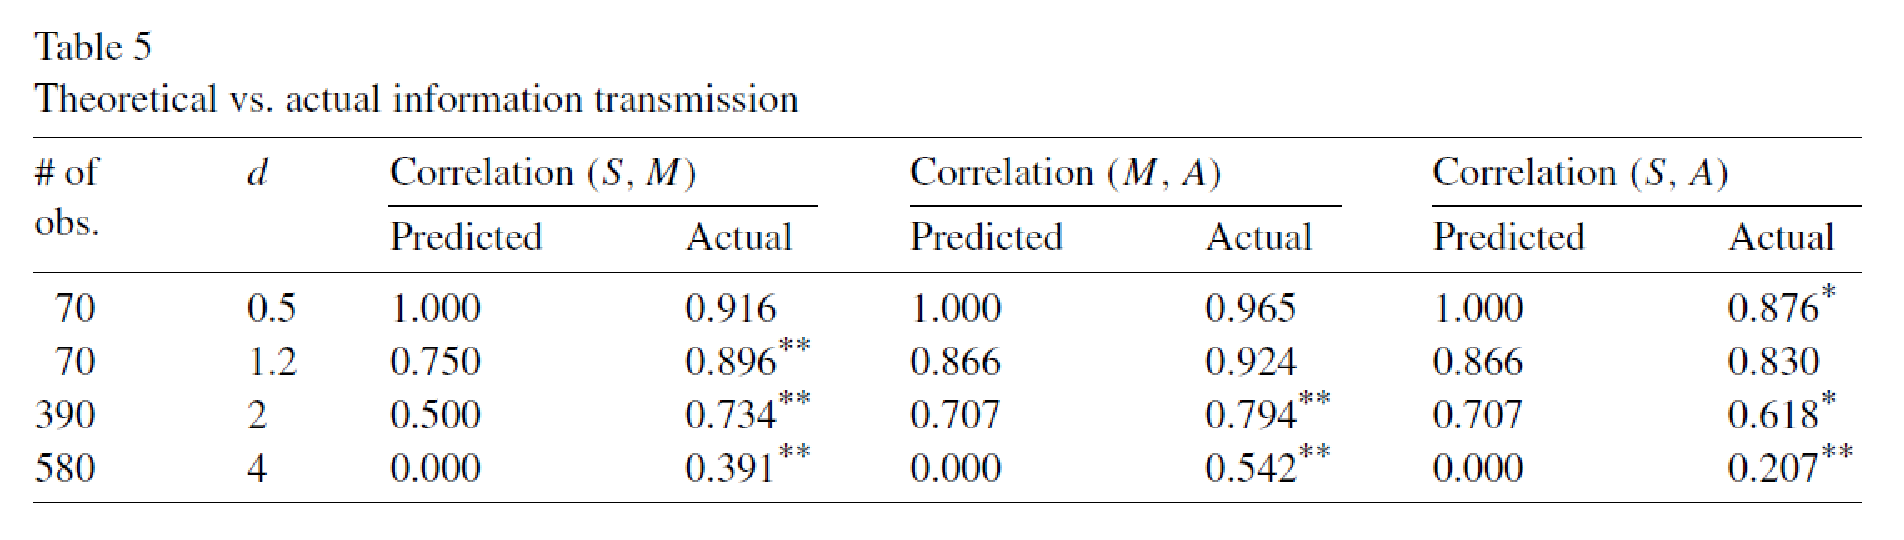
\includegraphics[width=3.0in]{images/cw2006Tbl5.eps}\end{center}
	\begin{itemize}
		\item Comparative statics are in the theoretical direction
		\item But there is greater correlation than predicted in non-perfect alignment games
		\item Implies more truth-telling than optimal
	\end{itemize}
\end{frame}

\begin{frame}{Cai \& Wang (GEB 2006)}
	\begin{itemize}
		\item In order to explain the data the authors fit two explanatory behavioral models
		\begin{enumerate}
			\item Quantal-Response Equilibrium

			(McKelvey \& Palfrey EE 1995, GEB 1998)
			\item Level-$k$ model (baseline honesty)

			(Nagel AER 1995; Stahl \& Wilson GEB 1995; Costa-Gomes et al EMA 2001; Crawford AER 2003)
		\end{enumerate}
	\end{itemize}
\end{frame}


\begin{frame}{Cai \& Wang (GEB 2006)}
	\begin{itemize}
		\item Level-$k$ model:
		\begin{enumerate}
			\setcounter{enumi}{-1}
			\item Sender honest $m_0=\theta$; Receiver Honest $x_0=m$
			\item $m_1=\theta+d ; x_1=m-d$
			\item $m_2=\theta+2 d ; x_1=m-2 d$
			$$\vdots$$
			\item[k.]  $m_k=\theta+2 k ; x_k=m-k d$
		\end{enumerate}
		\item Cai \& Wang adapt this hierarchy to their data and estimate the type distribution
	\end{itemize}
\end{frame}

\begin{frame}{Cai \& Wang (GEB 2006)}
\begin{center}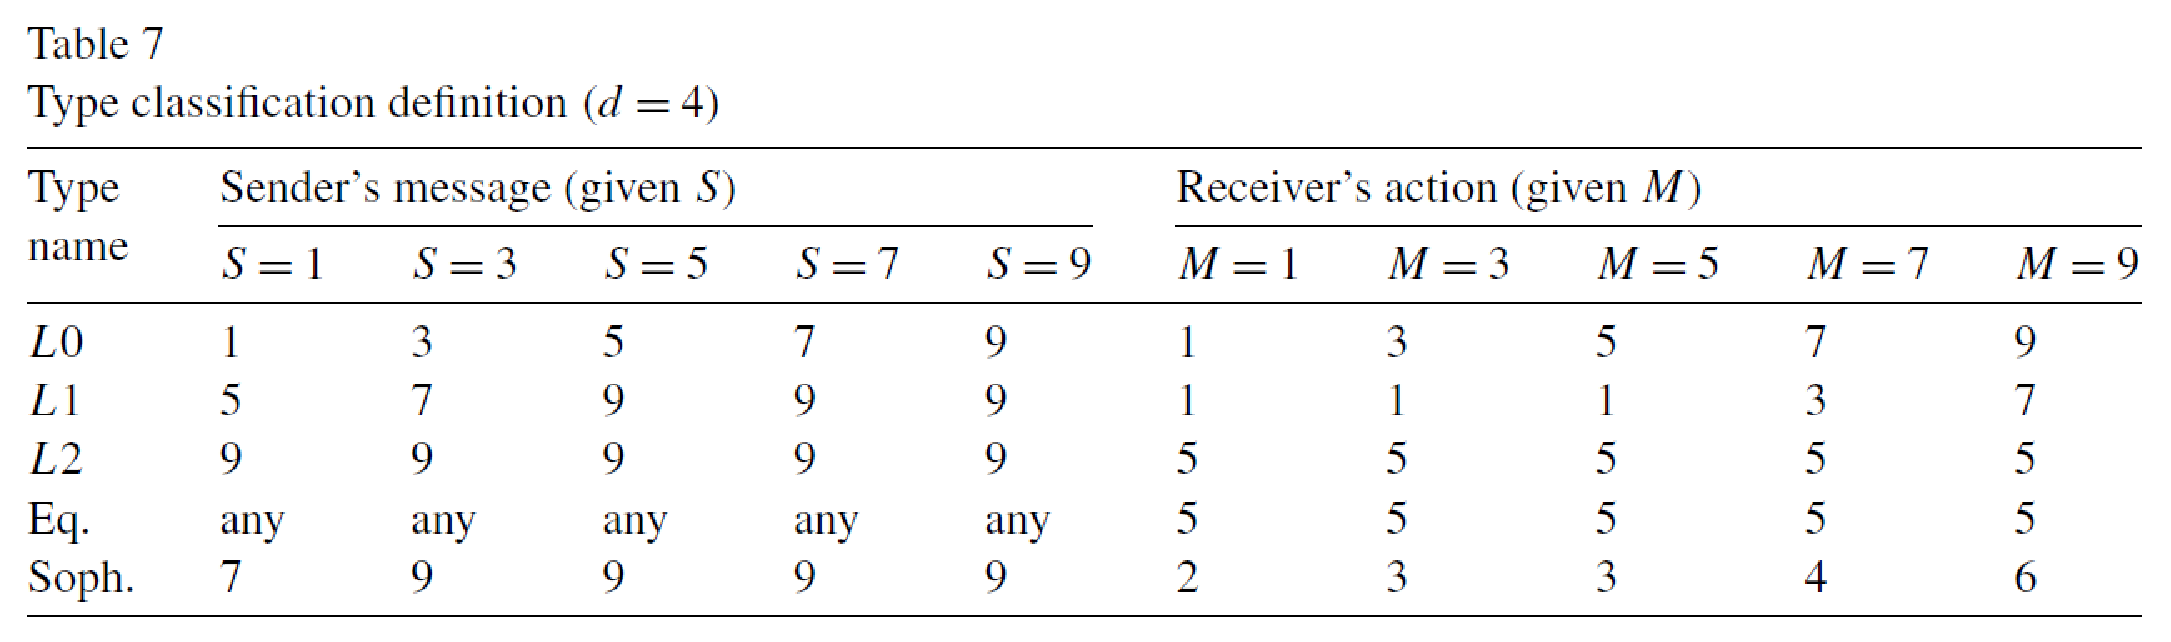
\includegraphics[width=4.0in]{images/cw2006Tbl7.eps}\end{center}
\end{frame}
\begin{frame}{Cai \& Wang (GEB 2006)}
\begin{center}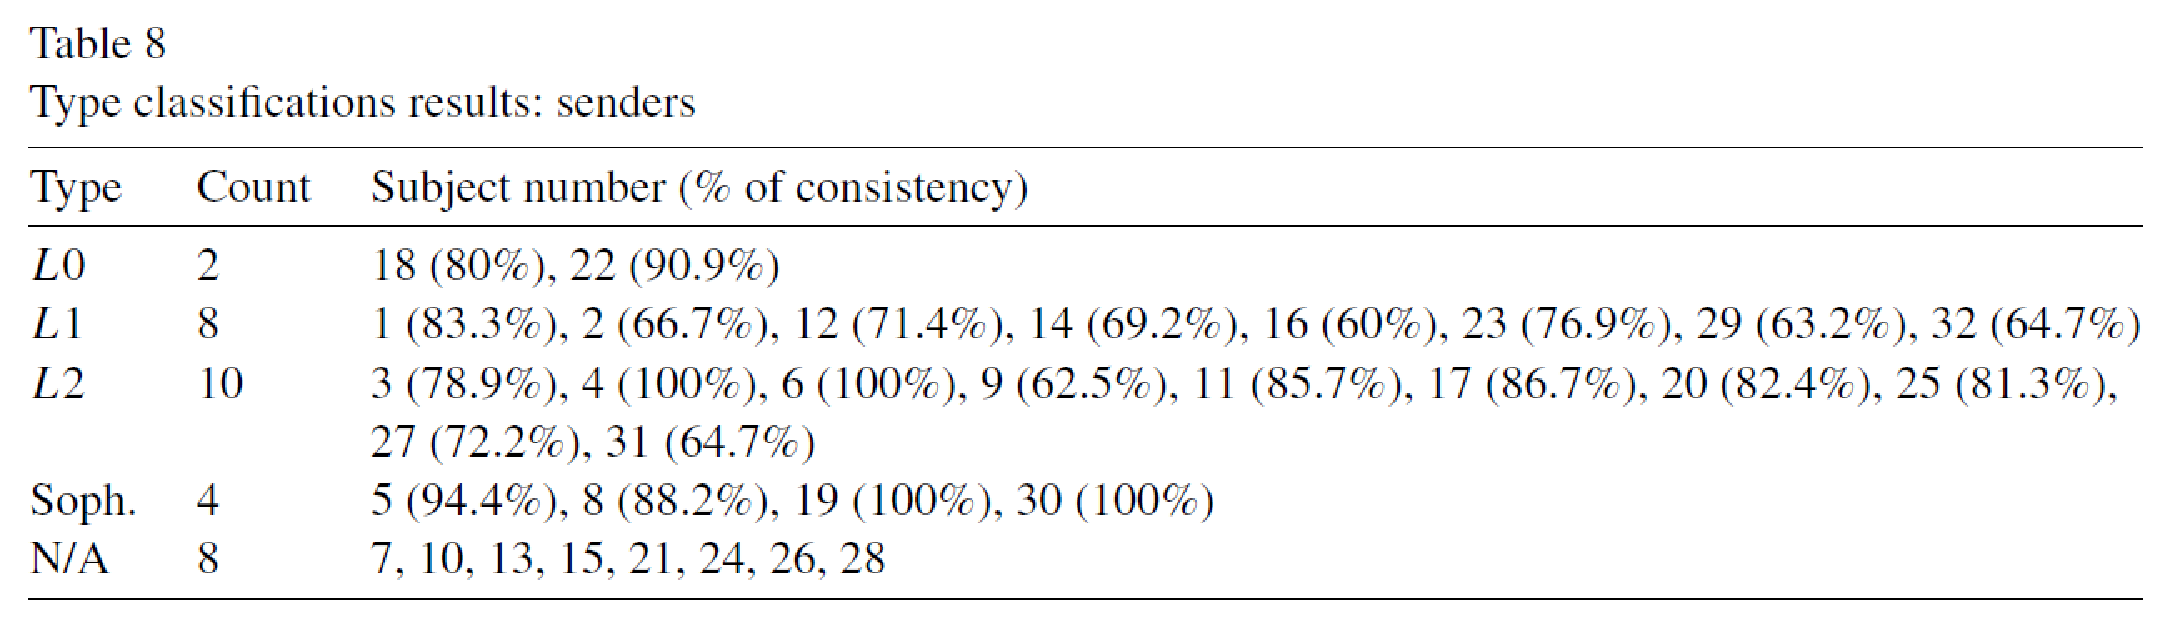
\includegraphics[width=4.0in]{images/cw2006Tbl8.eps}\end{center}
\end{frame}
\begin{frame}{Cai \& Wang (GEB 2006)}
\begin{center}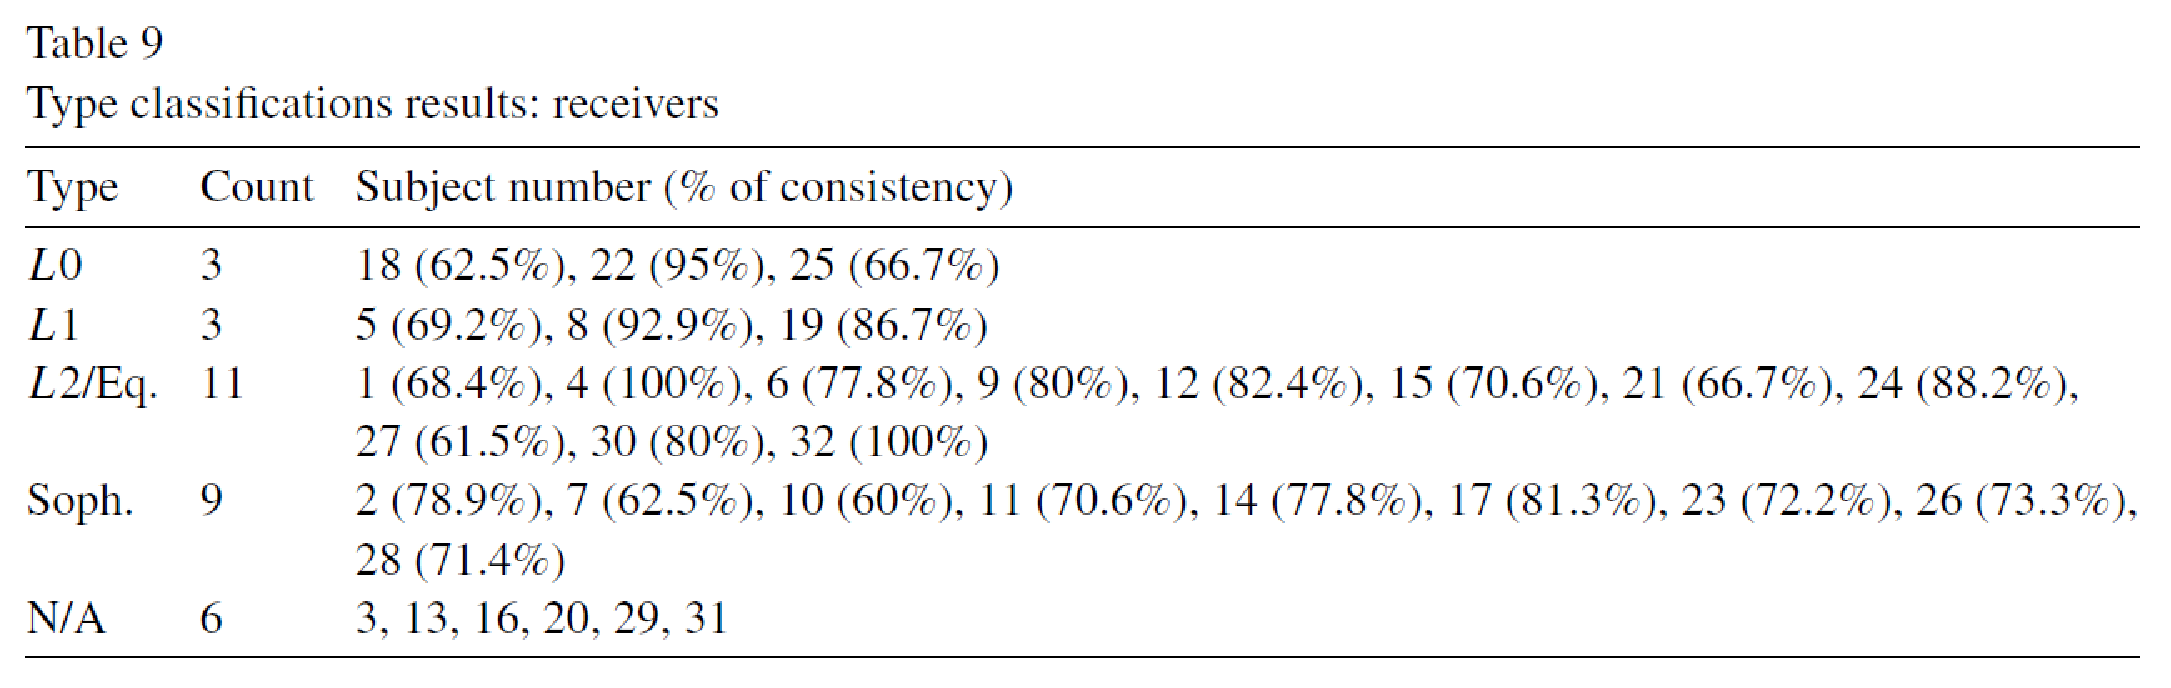
\includegraphics[width=4.0in]{images/cw2006Tbl9.eps}\end{center}
\end{frame}

\begin{frame}{Cai \& Wang (GEB 2006)}
Estimate following QRE model:
			$$
      p(\theta,m)=\Pr\left\{m\left| \theta\right. \right\}=
      \frac{\exp \left\{\lambda\cdot \hat{u}_\theta(m)\right\}}
      {\sum_{m^\prime\in M}\exp\left\{\lambda\cdot \hat{u}_{\theta}(m^\prime)\right\}}$$
			and
			$$
      q(m,x)=
			\Pr\left\{x\left| m\right. \right\}=
			\frac{\exp\left\{\lambda\cdot \hat{v}_m(x)\right\} }{      \sum_{x^\prime\in X} \exp\left\{\lambda\cdot \hat{v}_{m}(x^\prime)\right\}
      }
      $$
        where
      $$
      \hat{u}_\theta(m)=\sum_{x\in X} q(m,x) u(x,\theta)
      $$
			$$
      \hat{v}_m(x)=\sum_{\theta\in \Theta} r(\theta\left| m\right. ) v(x,\theta )
      $$
			with Bayesian posterior:
			$$
      r(\theta\left| m\right. )=\frac{p(\theta,m)}{\sum_{\theta^\prime\in\Theta} p(\theta^\prime,m)}
      $$

\end{frame}

\begin{frame}{Cai \& Wang (GEB 2006)}
	\begin{center}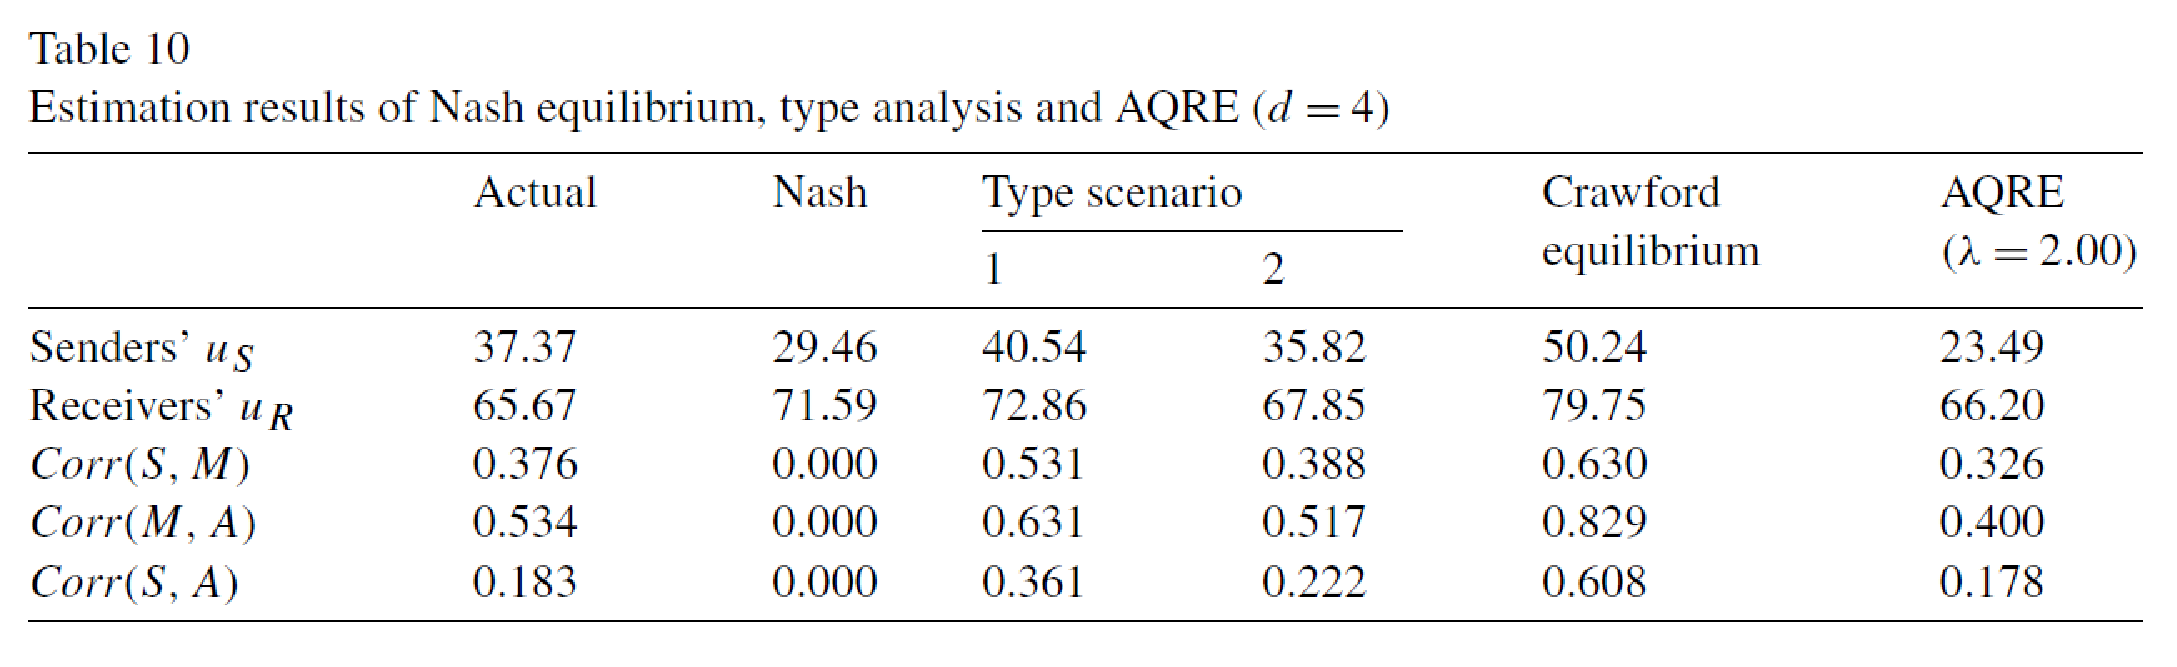
\includegraphics[width=4.0in]{images/cw2006Tbl10.eps}\end{center}
\end{frame}

\begin{frame}{Cai \& Wang (GEB 2006)}
	\begin{itemize}
		\item Main contribution here is in estimating a level-$k$ hierarchy with a focal level-$0$ behavior
		\item Both the QRE and level-$k$ models are explanatory models
		\item Can not pick easily between them
		\item Also, do not know the payoff effects from guilt, other-regarding, etc.
	\end{itemize}
\end{frame}

\section{Gneezy(2005)}
\begin{frame}{Gneezy (2005)}
	\begin{itemize}
		\item Two Roles: Senders \& Receivers
    \item Two Options A and B
	\end{itemize}
\end{frame}

\section{Gneezy(2005)}
\begin{frame}{Gneezy (2005)}
	\begin{itemize}
		\item Sender finds out the payoffs to the division of a pie:
		\begin{enumerate}[A]
			\item You get \$5, the other player gets \$15
			\item You get \$15, the other player gets \$5
		\end{enumerate}
		\item The sender then chooses a message from:
		\begin{enumerate}[a]
			\item ``Option A will earn you more money than Option B''
			\item ``Option B will earn you more money than Option A''
		\end{enumerate}
		\item Finally the receiver gets the message and makes a choice from \emph{A} and \emph{B}
	\end{itemize}
\end{frame}

\begin{frame}{Gneezy (2005)}
	\begin{itemize}
		\item Treatments are:

		\begin{tabular}{lccc}\hline
		& & \multicolumn{2}{c}{Payoff to:}\\ \cline{3-4}
		Treatment & Option & Sender & Receiver \\ \hline
		1		  &   A  & 5 & 6  \\
				  &   B  & 6 & 5  \\
		2		  &   A  & 5 & 15 \\
				  &   B  & 6 & 5  \\
		3		  &   A  & 15 & 5 \\
				  &   B  & 5 & 15 \\ \hline
		\end{tabular}
	\end{itemize}
\end{frame}
\begin{frame}{Gneezy (2005)}
	\begin{itemize}
		\item Majority of the messages suggestions are followed (approximately 80\%)
		\item Also run a dictator game treatment where the Sender subject just chooses the outcome from the outcomes $A$ and $B$
		\item Idea here is to look at preferences over dishonesty
	\end{itemize}
\end{frame}

\begin{frame}{Gneezy (2005)}
	\begin{center}
		\begin{tabular}{lccc}\hline
		& \multicolumn{3}{c}{Selfish Allocation B }\\ \cline{2-4}
		Game & (5,6) vs (6,5) & (5,15) vs (6,5) & (5,15) vs (15,5) \\ \hline
		Cheap Talk &   $0.36$  & $0.17$ & $0.52$  \\
		Dictator   &   $0.66$  & $0.42$ & $0.90$  \\ \hline
		\end{tabular}
	\end{center}

	\begin{itemize}
		\item So there is an aversion to deception in communication here.
		\item 38\% of the subjects would rather be honest than get \$10 extra for themselves (\$8 if you factor in receiver behavior)
		\item Statistically significant differences across Game.
	\end{itemize}
\end{frame}

\begin{frame}{Gneezy (2005)}
	\begin{itemize}
		\item Receivers do not know the possible set of states
		\item Subsequent experiments have shown that some of the ``honesty'' may be strategic
    \item Results have been replicated with honesty between the subject and experimenter (see Fischbacher and F\"ollmi-Heusi, JEEA 2013)
	\end{itemize}
\end{frame}

\begin{frame}{Fischbacher and F\"ollmi-Heusi, JEEA 2013}
\includegraphics<1>[width=1.0\textwidth]{images/Fischbacher2011.pdf}
\end{frame}

\section{Wang, Spezio \& Camerer (AER 2010))}
\begin{frame}{Wang, Spezio \& Camerer (AER 2010)}
	\begin{itemize}
		\item Cai \& Wang (2006) with:
		\begin{itemize}
			\item Eye-tracking
			\item Pupil Dilation
			\item Reaction times
		\end{itemize}
		\item Preferences are again
				$$u^R(x,\theta)=C_R-a\cdot \left|x-\theta\right|^{1.4}$$
				and for the sender are:
				$$v^S(x,\theta;d)=C_S-a\cdot \left|x+d-\theta\right|^{1.4}$$
	\end{itemize}
\end{frame}

\begin{frame}{Wang, Spezio \& Camerer (AER 2010)}
	\begin{itemize}
		\item Caltech undergrads
		\item Within-subject design
		\item Two senders were eye-tracked
		\item Six subjects in a session
		\item 45 rounds
		\item Six sessions
		\item Perturb payoffs to stop memory effects
	\end{itemize}
\end{frame}
\begin{frame}{Wang, Spezio \& Camerer (AER 2010)}
\begin{center}
\includegraphics<1>[height=0.8\textheight]{images/wsc2010Fig1.eps}
\includegraphics<2>[height=0.8\textheight]{images/wsc2010Fig2.eps}
\includegraphics<3>[height=0.8\textheight]{images/wsc2010Fig3.eps}
\end{center}
\end{frame}

\begin{frame}{Wang, Spezio \& Camerer (AER 2010)}
	\begin{itemize}
		\item Estimate the sender's level types using a spiked-logit model.
		\begin{itemize}
			\item $(1-\epsilon)$ probability of playing level-$k$
			\item $\epsilon$  probability of QRE-type-model around level-$k$ strategy/beliefs with free parameter $\lambda$
		\end{itemize}
		\item Estimate is a probability of being each level-$k$ type $\mathbf{p}$, $\epsilon$ and $\lambda$
		\item Estimations are by subject
	\end{itemize}
\end{frame}

\begin{frame}{Wang, Spezio \& Camerer (AER 2010)}
	\begin{center}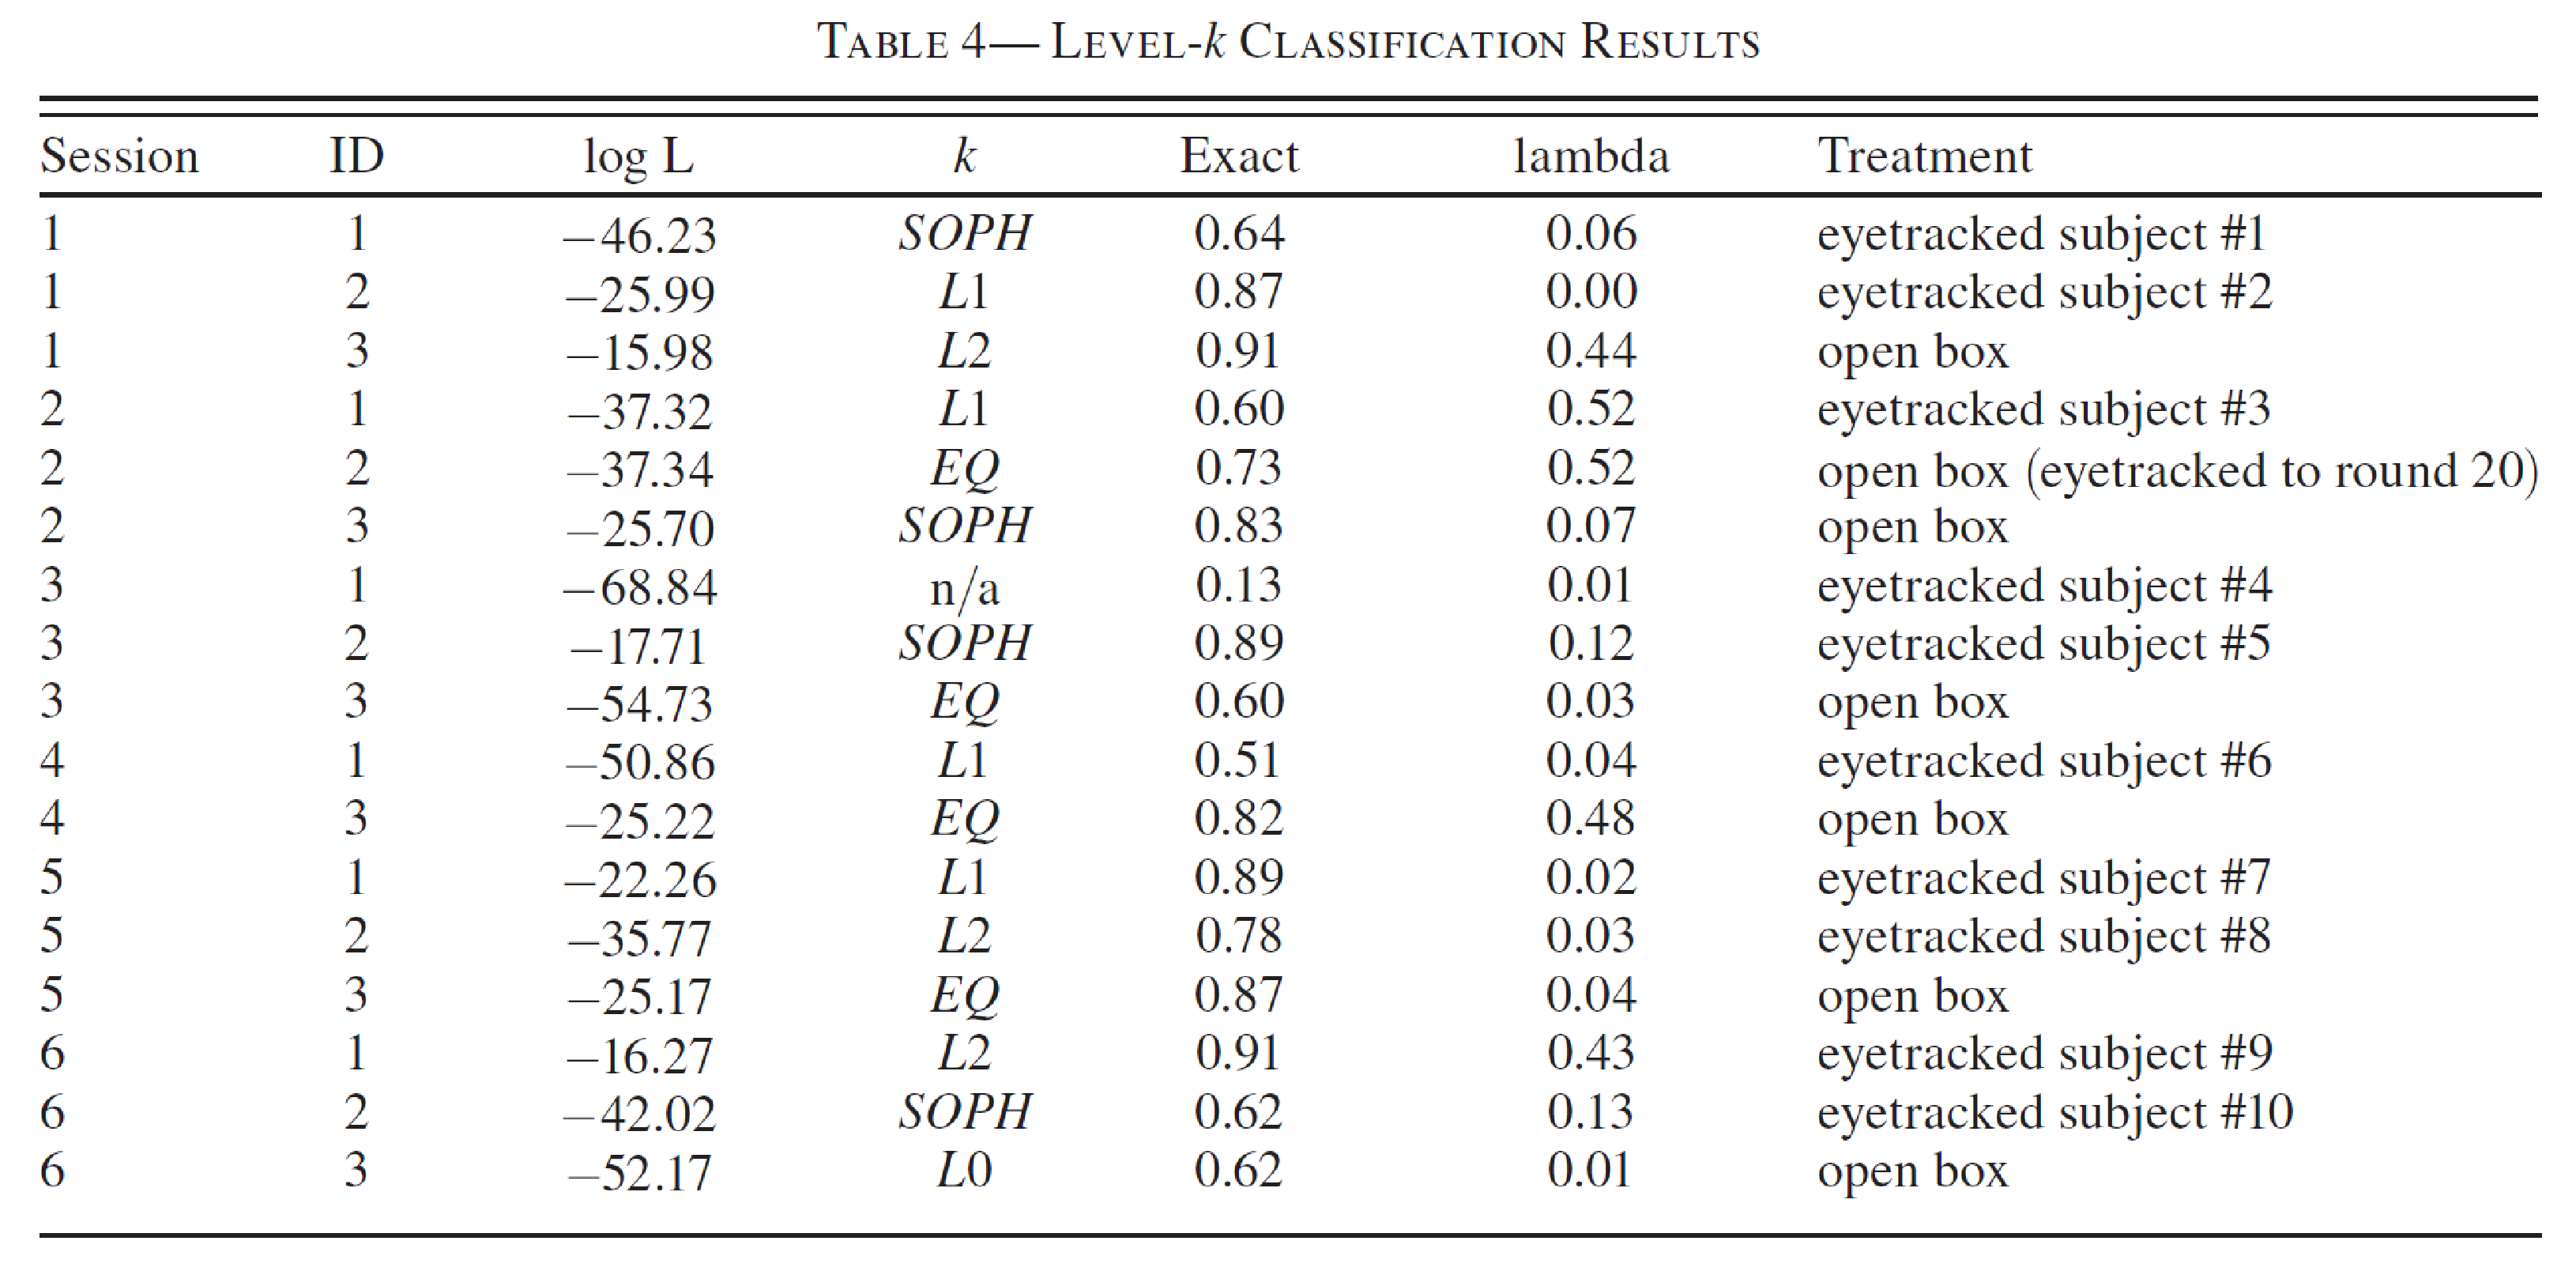
\includegraphics[width=4.0in]{images/wsc2010Tbl4.eps}\end{center}
	\begin{itemize}
	\item Mostly above 60\% probability on type
	\item Mix of behavioral types approximately similar to Cai \& Wang
	\end{itemize}
\end{frame}
\begin{frame}{Eye-Lookup Lengths \only<1>{Level 1 $b=1$}\only<2>{Level 2 $b=1$}\only<3>{Level 1 $b=2$}\only<4>{Level 2 $b=2$}}
\includegraphics<1>[width=1.0\textwidth]{images/wsc2010Fig4.eps}
\includegraphics<2>[width=1.0\textwidth]{images/wsc2010Fig5.eps}
\includegraphics<3>[width=1.0\textwidth]{images/wsc2010Fig6.eps}
\includegraphics<4>[width=1.0\textwidth]{images/wsc2010Fig7.eps}
\end{frame}
\begin{frame}{Wang, Spezio \& Camerer (AER 2010)}
	\begin{itemize}
		\item Subject senders do not spend enough time considering receiver's payoffs
		\item Level-estimations are broadly confirmed in consideration of own payoff lookups
	\end{itemize}
\end{frame}
\begin{frame}{Wang, Spezio \& Camerer (AER 2010)}
	\begin{itemize}
		\item Pupil dilation and eye-movements can be used to predict deceptive messages
		\item Conclude that their estimated model of behavior can do 20\% better than receivers at figuring out the problem
		\item Again, no real information on other-regarding concerns
		\item Not really sure on the economic significance of this part
		\item Main take-away seems to be further validation of the level-$k$ behavioral model with non-choice data
	\end{itemize}
\end{frame}

\end{document}
